
%% bare_jrnl.tex
%% V1.4b
%% 2015/08/26
%% by Michael Shell
%% see http://www.michaelshell.org/
%% for current contact information.
%%
%% This is a skeleton file demonstrating the use of IEEEtran.cls
%% (requires IEEEtran.cls version 1.8b or later) with an IEEE
%% journal paper.
%%
%% Support sites:
%% http://www.michaelshell.org/tex/ieeetran/
%% http://www.ctan.org/pkg/ieeetran
%% and
%% http://www.ieee.org/

%%*************************************************************************
%% Legal Notice:
%% This code is offered as-is without any warranty either expressed or
%% implied; without even the implied warranty of MERCHANTABILITY or
%% FITNESS FOR A PARTICULAR PURPOSE! 
%% User assumes all risk.
%% In no event shall the IEEE or any contributor to this code be liable for
%% any damages or losses, including, but not limited to, incidental,
%% consequential, or any other damages, resulting from the use or misuse
%% of any information contained here.
%%
%% All comments are the opinions of their respective authors and are not
%% necessarily endorsed by the IEEE.
%%
%% This work is distributed under the LaTeX Project Public License (LPPL)
%% ( http://www.latex-project.org/ ) version 1.3, and may be freely used,
%% distributed and modified. A copy of the LPPL, version 1.3, is included
%% in the base LaTeX documentation of all distributions of LaTeX released
%% 2003/12/01 or later.
%% Retain all contribution notices and credits.
%% ** Modified files should be clearly indicated as such, including  **
%% ** renaming them and changing author support contact information. **
%%*************************************************************************


% *** Authors should verify (and, if needed, correct) their LaTeX system  ***
% *** with the testflow diagnostic prior to trusting their LaTeX platform ***
% *** with production work. The IEEE's font choices and paper sizes can   ***
% *** trigger bugs that do not appear when using other class files.       ***                          ***
% The testflow support page is at:
% http://www.michaelshell.org/tex/testflow/



%\documentclass[journal,draft,onecolumn]{IEEEtran}
\documentclass[journal]{IEEEtran}
% *** GRAPHICS RELATED PACKAGES ***
%
\ifCLASSINFOpdf
  % \usepackage[pdftex]{graphicx}
  % declare the path(s) where your graphic files are
  % \graphicspath{{../pdf/}{../jpeg/}}
  % and their extensions so you won't have to specify these with
  % every instance of \includegraphics
  % \DeclareGraphicsExtensions{.pdf,.jpeg,.png}
\else
  % or other class option (dvipsone, dvipdf, if not using dvips). graphicx
  % will default to the driver specified in the system graphics.cfg if no
  % driver is specified.
  % \usepackage[dvips]{graphicx}
  % declare the path(s) where your graphic files are
  % \graphicspath{{../eps/}}
  % and their extensions so you won't have to specify these with
  % every instance of \includegraphics
  % \DeclareGraphicsExtensions{.eps}
\fi

\usepackage{lineno,hyperref}


%% The amssymb package provides various useful mathematical symbols
\usepackage{amssymb}
\usepackage{framed,multirow}
\usepackage{url,lineno,microtype}
\usepackage{mathrsfs,bm} % Notacion de transformadas
\usepackage{amsmath}
\usepackage{amsfonts,eucal}
\usepackage[normalem]{ulem}

\usepackage{epsfig}
\usepackage{epstopdf}
\usepackage{booktabs}
\usepackage{adjustbox}
\usepackage[]{subfigure}
\usepackage{lineno}

%\usepackage{tikz}
\usepackage{pgfplots}
%\usetikzlibrary{shadings}
%\pgfplotsset{compat=1.16}
%\usetikzlibrary{arrows,shapes,shadows,calc,decorations.pathreplacing,positioning}
%\usetikzlibrary{spy}
\usepgfplotslibrary{fillbetween}

\usepackage{times}
%\usepackage[titletoc,toc,title]{appendix}
\usepackage{natbib}
\usepackage{float}
\usepackage[ruled,linesnumbered]{algorithm2e}
\usepackage{array}
\usepackage{color}
\usepackage[capitalize]{cleveref}
\usepackage{enumerate,multirow}
\usepackage{lineno}


%%Defining some useful variables 
\providecommand{\promedd}[2]{\mathbb{E}_{#1}\!$\left\{#2\right\}$}% operador de promedio
\providecommand{\ve}[1]{{\bm{#1}}}%
\providecommand{\tr}[1]{{\operatorname{tr}$\left({#1}\right)$}}
\providecommand{\mat}[1]{{\bm{#1}}} %
\providecommand{\var}[1]{${\operatorname{var}}\left\{#1\right\}$}
\newcommand{\Real}{\mathbb{R}}
\newcommand{\N}{\mathbb{N}}
\newcommand{\Z}{\mathbb{Z}}

\DeclareMathOperator{\subconj}{\negthinspace\subset\negthinspace }
\DeclareMathOperator{\en}{\!\,\in\!\,}
\DeclareMathOperator{\igual}{\!\,=\!\,}
\DeclareMathOperator{\dist}{\operatorname{d}}
\DeclareMathOperator{\xx}{\negthickspace\times\negthickspace}
\providecommand{\s}[1]{\negthinspace#1\negthinspace}%

\renewcommand{\refname}{\normalsize References}
\newcommand{\dif}[1]{\mathrm{d}#1}
\newcommand{\Erf}[1]{\mathrm{erf}\left(#1\right)}
\newcommand{\Cov}[1]{\mathrm{cov}\left(#1\right)}
\newcommand{\sign}[1]{\mathrm{sign}(#1)}
\newcommand{\phivec}{\boldsymbol{\phi}}
\newcommand{\muvec}{\boldsymbol{\mu}}
\newcommand{\wfunc}[1]{\textnormal{w}(#1)}
\providecommand{\ve}[1]{{\mathbf{#1}}}

\DeclareMathOperator{\vecO}{vec} % vec operator
\providecommand{\mat}[1]{{\mathbf{#1}}}
\DeclareMathOperator{\cov}{cov} % Operator for the covariance
\DeclareMathOperator{\KL}{KL} % Operator for the KL divergence
\newcommand{\boldk}{\mathbf{k}} % kernel or covariance
\newcommand{\boldt}{\mathbf{t}} % kernel or covariance
\newcommand{\boldK}{\mathbf{K}} % kernel or covariance
\newcommand{\boldf}{\mathbf{f}} % outputs without noise
\newcommand{\boldB}{\mathbf{B}} % coregionalization matrix
\newcommand{\boldA}{\mathbf{A}} % matrix of coeffcients a_{qi}^r
\newcommand{\boldc}{\mathbf{c}} % matrix of coeffcients a_{qi}^r
\newcommand{\boldu}{\mathbf{u}} % vector for latent function
\newcommand{\bolda}{\mathbf{a}}
\newcommand{\boldm}{\mathbf{m}}
\newcommand{\boldv}{\mathbf{v}}
\newcommand{\boldV}{\mathbf{V}}
\newcommand{\boldW}{\mathbf{W}}
\newcommand{\boldY}{\mathbf{Y}}
\newcommand{\boldy}{\mathbf{y}}
\newcommand{\boldx}{\mathbf{x}}
\newcommand{\boldZ}{\mathbf{Z}}
\newcommand{\boldz}{\mathbf{z}}
\newcommand{\boldAtilde}{\mathbf{\widetilde{A}}}
\newcommand{\eye}{\mathbf{I}}   % identity matrix
\newcommand{\boldI}{\mathbf{I}} % identity matrix
\newcommand{\boldUpsi}{\bm{\Upsilon}}
\newcommand{\boldX}{\mathbf{X}} % The whole set of input vectors
\newcommand{\boldH}{\mathbf{H}} % The whole set of lag vectors
\newcommand{\inputSpace}{\mathcal{X}} % The input space
\newcommand{\params}{\bm{\theta}} % Parameters of LMC model
\newcommand{\veC}{\textbf{\hspace{-0.001in}:}} % Simplified version of the vec operator (vec = :)
\newcommand{\preci}{\mathbf{P}}% Precision for the Gaussians
\newcommand{\dataset}{{\cal D}} % dataset
\newcommand{\fracpartial}[2]{\frac{\partial #1}{\partial  #2}} % Fraction for partial derivatives
\newcommand{\gauss}{\mathcal{N}} % Gaussian density
\newcommand{\bolds}{\mathbf{s}}


\newcommand\redsout{\bgroup\markoverwith{\textcolor{red}{\rule[0.5ex]{2pt}{0.4pt}}}\ULon}
\providecommand{\roj}[1]{\textcolor{red}{\uwave{#1}}}
\providecommand{\ver}[1]{\textcolor{green}{\uwave{#1}}}
\providecommand{\gc}[1]{\textcolor{darkgray}{\uwave{#1}}}
\providecommand{\am}[1]{\textcolor[rgb]{0.1,0.5,0.0}{\upshape{#1}}}
% Leave a blank line between paragraphs instead of using \\

%Comments
\providecommand{\am}[1]{\textcolor[rgb]{0.1,0.5,0.0}{\upshape{#1}}}

\newcolumntype{C}[1]{>{\centering\let\newline\\\arraybackslash\hspace{0pt}}m{#1}}

\usepackage{pifont}% http://ctan.org/pkg/pifont
\newcommand{\cmark}{\ding{51}}%
\newcommand{\xmark}{\ding{55}}%
\usetikzlibrary{bayesnet}

% correct bad hyphenation here
\hyphenation{op-tical net-works semi-conduc-tor}


\begin{document}
%
% paper title
% Titles are generally capitalized except for words such as a, an, and, as,
% at, but, by, for, in, nor, of, on, or, the, to and up, which are usually
% not capitalized unless they are the first or last word of the title.
% Linebreaks \\ can be used within to get better formatting as desired.
% Do not put math or special symbols in the title.
\title{Correlated Chained Gaussian Processes with Multiple Annotators}
%
%
% author names and IEEE memberships
% note positions of commas and nonbreaking spaces ( ~ ) LaTeX will not break
% a structure at a ~ so this keeps an author's name from being broken across
% two lines.
% use \thanks{} to gain access to the first footnote area
% a separate \thanks must be used for each paragraph as LaTeX2e's \thanks
% was not built to handle multiple paragraphs
%

\author{J. Gil-Gonz\'alez,
        J. Giraldo,
        A. \'Alvarez-Meza, A. Orozco-Guti\'errez, and
        and~M.~\'Alvarez-L\'opez% <-this % stops a space
\thanks{J. Gil-Gonz\'alez and A. Orozco are with the Faculty of Engineering, Universidad Tecnol\'ogica de Pereira, Colombia, 660003, e-mail:jugil@utp.edu.co}% <-this % stops a space
\thanks{J. Giraldo and M. \'Alvarez are with Department of Computer Science, University of Sheffield, UK.}% <-this % stops a space
\thanks{A. \'Alvarez is with  Universidad Nacional de Colombia sede Manizales, Colombia}}
%\thanks{Manuscript received April 19, 2005; revised August 26, 2015.}}

% note the % following the last \IEEEmembership and also \thanks - 
% these prevent an unwanted space from occurring between the last author name
% and the end of the author line. i.e., if you had this:
% 
% \author{....lastname \thanks{...} \thanks{...} }
%                     ^------------^------------^----Do not want these spaces!
%
% a space would be appended to the last name and could cause every name on that
% line to be shifted left slightly. This is one of those "LaTeX things". For
% instance, "\textbf{A} \textbf{B}" will typeset as "A B" not "AB". To get
% "AB" then you have to do: "\textbf{A}\textbf{B}"
% \thanks is no different in this regard, so shield the last } of each \thanks
% that ends a line with a % and do not let a space in before the next \thanks.
% Spaces after \IEEEmembership other than the last one are OK (and needed) as
% you are supposed to have spaces between the names. For what it is worth,
% this is a minor point as most people would not even notice if the said evil
% space somehow managed to creep in.



% The paper headers
\markboth{Journal of \LaTeX\ Class Files,~Vol.~14, No.~8, August~2015}%
{Shell \MakeLowercase{\textit{et al.}}: Bare Demo of IEEEtran.cls for IEEE Journals}
% The only time the second header will appear is for the odd numbered pages
% after the title page when using the twoside option.
% 
% *** Note that you probably will NOT want to include the author's ***
% *** name in the headers of peer review papers.                   ***
% You can use \ifCLASSOPTIONpeerreview for conditional compilation here if
% you desire.




% If you want to put a publisher's ID mark on the page you can do it like
% this:
%\IEEEpubid{0000--0000/00\$00.00~\copyright~2015 IEEE}
% Remember, if you use this you must call \IEEEpubidadjcol in the second
% column for its text to clear the IEEEpubid mark.



% use for special paper notices
%\IEEEspecialpapernotice{(Invited Paper)}




% make the title area
\maketitle


\linenumbers

% As a general rule, do not put math, special symbols or citations
% in the abstract or keywords.
\begin{abstract}
A dataset to train a supervised learning algorithm comprises features and their corresponding labels. The labeling process is usually carried out by an expert, which provides the ground truth/gold standard for each sample. However, in many real-world applications, instead of such a gold standard, we usually have access to annotations provided by crowds, which hold different and unknown expertise levels. Thus, Learning from crowds is a subject undergoing intense study, and its main aim is to face different machine learning paradigms in the presence of multiple annotators. Most state-of-the-art approaches reside on two key assumptions: i) the labeler’s performance does not depend on the input feature space, and ii) independence among the annotators is imposed. Accordingly, we introduce the chained Gaussian processes--(CGPMA) model and the correlated chained Gaussian processes--(CCGPMA) model to deal with multi-labelers problems. Namely, CGPMA allows modeling each annotator's performance as a function of the input space. Similarly, CCGPMA is an extension of CGPMA to exploit correlations among the labelers' answers. Experimental results devoted to regression and classification show that our CCGPMA achieves suitable performances from inconsistent labelers, even if the gold standard is not available.
\end{abstract}

% Note that keywords are not normally used for peerreview papers.
\begin{IEEEkeywords}
Multiple annotators, Chained Gaussian Processes, Classification, Regression.
\end{IEEEkeywords}

% For peer review papers, you can put extra information on the cover
% page as needed:
% \ifCLASSOPTIONpeerreview
% \begin{center} \bfseries EDICS Category: 3-BBND \end{center}
% \fi
%
% For peerreview papers, this IEEEtran command inserts a page break and
% creates the second title. It will be ignored for other modes.
\IEEEpeerreviewmaketitle



\section{Introduction}

\IEEEPARstart{S}{upervised} learning requires the acquisition of high-quality training sets. The labeling process is performed by a domain expert, which is supposed to provide the absolute true label (termed gold standard/ground truth) \citep{zhang2019crowdsourced}. However, the experts are scarce; their time is expensive; the labeling task is tedious and time-consuming. Therefore, the gold standard's availability is hardly feasible for many real-world applications \citep{liu2020truth}. An alternative is to distribute the labeling task to multiple heterogeneous annotators (also known as labelers or sources), where each labeler annotates part of the whole dataset by providing its version (possibly noisy) of the hidden ground truth \cite{kara2015modeling}. Those annotations can be collected in several ways. For instance, in \cite{raykar2010learning}, the sources are physicians who make a diagnosis about the presence of cancer, based on the analysis of medical images. Likewise, in \cite{zhu2019unsupervised}, the labelers are algorithms that measure the QT interval in an electrocardiogram (ECG) signal. Besides, crowdsourcing platforms such as Amazon Mechanical Turk (AMT)\footnote{https://www.mturk.com/} are becoming a valuable tool to obtain labels from multiple sources for large datasets in an efficient way (regarding labeling time). The attractiveness of these platforms lies in that at a low cost, it is possible to obtain suitable quality labels that, in some cases, can compete with those provided by experts~\cite{snow2008cheap}. 

Accordingly, in a multi-labeler setting, each input feature is matched with multiple annotations provided by different sources with unknown and diverse expertise. Thus, it is clear that such a problem cannot be faced with traditional supervised learning algorithms \cite{tao2018domain,wang2016bi}. Taking the above into account, the question is how to perform predictions with information from multiple annotators? Such a question has been addressed by an area named \emph{Learning from crowds}, which is undergoing intense study in the machine learning context \cite{groot2011learning}. \emph{Learning from crowds} offers two options to deal with multi-labeler problems data: \textit{i)} to adapt the labels from multiple annotators or \textit{ii)} to accommodate the supervised learning techniques~\cite{rizos2020average}. 

The first approach is known in the literature as ``Label aggregation'' or ``Truth inference''. It comprises the computation of a single hard label per sample as an estimation of the unknown ground truth. These hard labels are then used to feed a standard supervised learning algorithm~\cite{morales2019scalable}. The most straightforward approach is the so-called majority voting--(MV); it has been used in different multi-labeler problems due to its simplicity~\cite{zhang2014imbalanced}. However, MV assumes homogeneity in annotators' reliability, which is hardly feasible in real applications, e.g., experts vs. spammers. Furthermore, the consensus is profoundly impacted by incorrect labels and outliers~\cite{kara2015modeling}. Conversely, more elaborated models have been considered to improve the estimation of the correct tag. For example, authors in \cite{dawid1979maximum} use an Expectation-Maximization (EM) algorithm to compute each labeler's reliability and infer the ground truth models. Besides, the work in \cite{zhang2014imbalanced} gives an estimation of the actual label by facing the problem of imbalanced labeling.  

The second approach comprises the modification of supervised learning algorithms to jointly train the supervised learning algorithm and the annotators' behavior. It has been shown that such strategies lead to better performance compared to the ones belonging to Label aggregation. Namely, the features used to train the learning algorithm provides valuable information to puzzle out the ground truth~\cite{ruiz2019learning}. The most representative work in this area is the exposed in \cite{raykar2010learning}, which offers an EM-based framework to learn the parameters of a logistic regression classifier and model the annotators' behavior by computing their sensitivities and specificities. This work has inspired several models in the context of multi-labelers scenarios. For instance, for binary classification \cite{rodrigues2014gaussian,ruiz2019learning}, multi-class classification \cite{morales2019scalable,gonzalez2015automatic}, regression \cite{groot2011learning,rodrigues2017learning}, and sequence labeling~\cite{rodrigues2014sequence}. Furthermore, in the last years, some works have faced the multi-labeler problem using deep learning approaches \cite{albarqouni2016aggnet,rodrigues2018deep,guan2018said}. Chiefly, the idea of this kind of approach is to design an extra layer to code multiple annotators' information. 

From the above, we can note an increasing interest in developing algorithms to deal with data from multiple labelers. Notwithstanding, as was analyzed in \cite{g2019machine}, there exist some problems that are not entirely solved; specifically, we are interested in the two following: \textit{i)} to code the relationship between the input features and the labelers' behavior, and \textit{ii)} to reveal the annotators' interdependencies. Regarding the first assumption, to model the annotators' behavior, it is necessary to learn some parameters related to their performance. Such parameters include the accuracy \cite{rodrigues2013learning}, the confusion matrix \cite{gonzalez2015automatic}, the error variance \cite{raykar2010learning}, and the bias \cite{rodrigues2017learning}. In the literature, we commonly find that the parameters are modeled as fixed points \cite{rodrigues2014gaussian} or as random variables \cite{morales2019scalable}, where it is considered that such parameters are homogeneous across the input data. The latter assumption is not correct since an expert makes decisions based not only on his/her expertise but also on the features observed from raw data \cite{raykar2010learning}. For the second assumption, it is widespread to consider independence among the annotators, aiming to reduce the complexity of the model~\cite{venanzi2014community}, or based on the fact that it is plausible to guarantee that each labeler performs the annotation process individually~\cite{tang2019leveraging}. Notwithstanding, this assumption is not entirely true since there may exist correlations among the annotators \cite{zhang2011learning}. For example, if the sources are humans, the independence assumption is hardly feasible because knowledge is a social construction; then, people's decisions will be correlated since they share information, communicate with each other, or belong to a particular school of thought~\cite{surowiecki2005wisdom,hahn2018communication}. On the other hand, if we consider that the sources are algorithms, where some of them gather the same math principle, there likely exists a correlation among their labels~\cite{zhu2019unsupervised}. Accordingly, the relaxation of this restriction can improve the ground truth estimation~\cite{g2019machine}.

Here, we propose a probabilistic framework based on Gaussian Processes--(GPs) to jointly build a prediction algorithm (regression and classification) and model the labelers' behavior as a function of the input features and taking into account annotators' interdependencies.\\
We perform an initial approach by applying the Chained GPs--(CGP) \cite{saul2016chained} model to the prediction problem with multiple annotators. CGPs are a Multi-GPs framework, where the parameters of an arbitrary likelihood function are modeled with multiple independent GPs (one GP per parameter). From the multiple annotators' point of view, the likelihood's parameters are related to the labelers' behavior. Hence, by using CGPs for multiple annotators (CGPMA), we are modeling each annotator's performance as a function of the input features, which coincides with one of this work aims; however, due to CGP uses independent GPs, the modeling of dependencies (or correlation) among individual labelers is missing.\\
Conversely, aiming to model such labelers' interdependencies, we introduce an extension to the CGPs named Correlated Chained GP for multiple annotators--(CCGPMA), which induces correlations between multiple GPs that model the likelihood's parameters. To this end, we take as a basis the ideas from a Multi-output GP--(MOGP) regression \cite{alvarez2012kernels}, where each output is coded as a weighted sum of shared latent functions via a semi-parametric latent factor model (SLFM) \cite{teh2005semiparametric}. Nevertheless, conversely to MOGP, we do not have multiple outputs but multiple functions chained to the parameters of a given likelihood. Hence, to introduce correlations among the parameters' functions, we suppose them to be generated from an SLFM of $Q$ latent functions, where each hidden function obeys a GP; thus, we are modeling the labelers' performance by taking into account interdependencies among them. The formulation of our CCGPs is based on the so-called inducing variables \cite{alvarez2010efficient} in combination with stochastic variational inference \cite{hoffman2013stochastic}, which make them scalable to large datasets. To the best of our knowledge, this is the first attempt to build a probabilistic approach that models both the interdependencies among the annotators and the relationship between the input features and the labelers' performance. Obtained results, using both simulated and real-world annotators, show how our methodology can deal with both regression and classification problems from multi-labelers data, outperforming state-of-the-art techniques.

The remainder is organized as follows. Section 2 exposes the related work and main contributions of the proposal. Section 3 describes the methods. Sections 4 and 5 present the experiments and discuss the results. Finally, Section 6 outlines the conclusions and future work.

\section{Related work and main contributions}

% In supervised learning with multiple annotators problems, each input sample is matched with a set of multiple labels, which are versions of an unknown true label; hence, this type of problem cannot be tackled with traditional supervised learning algorithms~\cite{ruiz2019learning}. Aiming to deal with multi-labeler settings, two options arise: \textit{i)} to adapt the labels from multiple annotators or \textit{ii)} to accommodate the supervised learning techniques~\cite{rizos2020average}. 

% The first approach is known in the literature as ``Label aggregation''. It comprises the extraction of a single hard label per sample, which is supposed to be an estimation of the unknown ground truth. These hard labels are then used to feed a standard supervised learning algorithm~\cite{morales2019scalable}. The most straightforward approach is the so-called majority voting--(MV); it has been used in different multi-labeler problems due to its simplicity~\cite{zhang2014imbalanced}. However, MV assumes homogeneity in annotators' reliability, which is hardly true in real-world applications, e.g., experts vs. spammers. Conversely, more elaborated models have been considered to improve the estimation of the correct tag. For example, authors in \cite{dawid1979maximum} use an Expectation-Maximization (EM) algorithm to compute each labeler's reliability and infer the ground truth models. Besides, the work in \cite{zhang2014imbalanced} gives an estimation of the actual label by facing the problem of imbalanced labeling.

% Regarding the second approach, it comprises the modification of supervised learning algorithms to jointly learn the classifier (regressor) parameters and the annotators' behavior. It has been shown that such strategies lead to better performance compared to the ones belonging to Label aggregation. Namely, the features used to train the learning algorithm provides valuable information to puzzle out the ground truth~\cite{ruiz2019learning}. The most representative work in this area is the exposed in \cite{raykar2010learning}, which offers an EM-based framework to learn the parameters of a logistic regression classifier and to model the annotators' behavior by computing their sensitivities and specificities. This work has inspired several models in the context of multi-labelers scenarios. For instance, for binary classification, authors in \cite{rodrigues2014gaussian} offer an extension based on Gaussian processes (GP) with Expectation-Propagation (EP) inference to deal with non-linearly separable data. Authors in \cite{ruiz2019learning} uses a GP classifier to learn the annotators' parameters using variational inference. Similarly, in \cite{morales2019scalable}, a sparse approximation of the previous model is introduced to make it scalable to large datasets. Conversely, the early work in \cite{raykar2010learning} has been extended to other supervised learning paradigms such as multi-class classification \cite{morales2019scalable,gonzalez2015automatic}, and regression \cite{groot2011learning,rodrigues2017learning}. Furthermore, in the last years, some works have faced the multi-labeler problem using deep learning \cite{albarqouni2016aggnet,rodrigues2018deep,guan2018said}. Chiefly, the idea of this kind of approach is to design an extra layer to code the information of multiple annotators. 

We note an increasing interest in developing algorithms to deal with data from multiple labelers. Notwithstanding, as was analyzed in \cite{g2019machine}, there exist some problems that are not entirely solved: \textit{i)} to code the relationship between the input features and the labelers' behavior, and \textit{ii)} to reveal the annotators' interdependencies. 

First, aiming to model the annotators' behavior, it is necessary to learn some parameters related to their performance. Such parameters include the accuracy \cite{rodrigues2013learning}, the confusion matrix \cite{gonzalez2015automatic}, the error variance \cite{raykar2010learning}, and the bias \cite{rodrigues2017learning}. In the literature, it is commonly founded that the parameters are modeled as fixed points \cite{rodrigues2014gaussian} or as random variables \cite{morales2019scalable}, where it is considered that such parameters are homogeneous across the input data. The latter assumption is wrong since an expert makes decisions based not only on his/her expertise but also on the features observed from raw data \cite{raykar2010learning}. The first attempt to analyze the relationship between the annotators' parameters and the input features is the work in \cite{zhang2011learning}. The authors propose an approach for binary classification with multiple labelers, where the input data is represented by some clusters using a Gaussian Mixtures Model--(GMM). Then, they assumed that for each cluster, the annotators exhibit a particular performance measured in terms of sensitivity and specificity. However, this labelers' model is not adequate because they do not consider the information from multiple experts as an input for the GMM, which could generate some regions where the labelers' parameters may vary. In \cite{yan2014learning}, the authors propose a binary classification algorithm that employs two approaches to code the annotators' performance as a function of the input space: a Bernoulli and a Gaussian distribution. The parameters of these distributions are computing via a Logistic regression scheme. Nonetheless, they assume a linear dependence between the labeler expertise and the input space, which may not be appropriate in real-world scenarios. For example, if we consider online annotators assessing some documents, they may have different labeling accuracy. Such differences may rely on whether they are more familiar with some issues than other \cite{wang2016bi}, which configures nonlinear behavior. Finally, \cite{xiao2013learning} offers a GP-based regression scheme with multiple annotators.  An additional GP is included to model the annotators' parameters as a nonlinear function of the input space. Nevertheless, such a model does not consider the uncertainty in the parameters \cite{bishop2006pattern}.

Now, the independence among the annotators is commonly used to reduce the complexity of the model \cite{venanzi2014community}, or based on the fact that it is plausible to guarantee that each labeler performs the annotation process individually \cite{tang2019leveraging}. Nevertheless, this is not entirely correct due to there may exist correlations among the annotators \cite{zhang2011learning}. For example, if the sources are humans, the independence assumption is hardly feasible because knowledge is a social construction; hence, people's decisions will be correlated when they share information, communicate with each other, or belong to a particular school of thought \cite{surowiecki2005wisdom,hahn2018communication}. Accordingly, the relaxation of this restriction could be used to improve the ground truth estimation \cite{g2019machine}. To the best of our knowledge, only two works gather the dependencies among the labelers. First,  authors in \cite{zhu2019unsupervised} expose an approach to deal with regression problems, where the labelers' behavior is addressed using a multivariate Gaussian distribution. Thus, the annotators' interdependencies are coded in the covariance matrix.  In \cite{gil2018learning}, authors propose a binary classification approach based on a weighted combination of classifiers, where each classifier models each annotator's response. In turn,  the weights are estimated by using a kernel alignment-based approach considering dependencies among the labelers. 

According to the related previously, we propose a framework based on GPs to face classification and regression settings with multiple annotators. Our proposal follows the line of the works in \cite{rodrigues2014gaussian,groot2011learning,ruiz2019learning,morales2019scalable,morales2019scalable1} in the sense that we are modeling the unknown ground truth trough a GP. However, while such approaches code the annotators' parameters as fixed points \cite{rodrigues2014gaussian,groot2011learning} or as random variables \cite{ruiz2019learning,morales2019scalable,morales2019scalable1}; we model them as random processes (GPs) aiming to take into account dependencies between the input space and the labelers' behavior. On the other hand, our CGPMA and CCGPMA share some similarities  \cite{yan2014learning,xiao2013learning}, due to these works assume dependencies between the input features and the labelers' performance. Besides, our CCGPMA is similar to approaches in \cite{zhu2019unsupervised,gil2018learning} because they assume the existence of dependencies among the annotators.
Nonetheless, in contrast to these approaches, our CCGPMA is the only approach that includes such assumptions to code the annotators' behavior. Finally, We highlight that due to our approach is capable to model inconsistent annotators, it is more robust to outliers compared with such models that do not consider the relationship between the input features and the labelers' behavior. Namely, CCGPMA can estimate the annotators' performance for every region in the input space; meanwhile, the other approaches estimate such performance as an average of some parameters \cite{rodrigues2017learning,morales2019scalable,ruiz2019learning}. Consequently, it is known that the average operator suffers under the presence of outliers \cite{kara2015modeling}. \cref{tab:SOA} summarizes the similarities and differences among our CGPMA, CCGPMA, and state-of-the-art approaches.

\begin{table*}[!tb]
	\centering
	\caption{Survey of relevant supervised learning models devoted to multiple annotators.}
	\resizebox{1\linewidth}{!}{
		\begin{tabular}{C{5cm}cC{4cm}cC{3cm}cC{3cm}cC{3cm}}\toprule
			Source && Data type && Modeling the annotator’s expertise && Expertise as a function of the input space && Modeling the annotators' interdependencies 
            \\\midrule
            \textit{Raykar et al., 2010} \cite{raykar2010learning} && Regression-Binary-Categorical && \cmark && \xmark && \xmark\\
            \textit{Zhang and Obradovic, 2011} \cite{zhang2011learning} && Binary && \cmark && \cmark && \xmark\\
            \textit{Xiao et al., 2013} \cite{xiao2013learning} && Regression && \cmark && \cmark && \xmark\\
            \textit{Yan et al., 2014} \cite{yan2014learning} && Binary && \cmark && \cmark && \xmark\\
            \textit{Wang and Bi, 2016} \cite{wang2016bi}&& Binary && \cmark && \cmark && \xmark\\
            \textit{Rodrigues et al., 2017} \cite{rodrigues2017learning} && Regression-Binary-Categorical && \cmark && \xmark && \xmark\\
            \textit{Gil-Gonzalez et al., 2018} \cite{gil2018learning} && Binary && \cmark && \xmark && \cmark\\
            \textit{Hua et al., 2018} \cite{hua2018collaborative} && Binary-Categorical && \cmark && \xmark && \xmark\\
            \textit{Ruiz et al., 2019} \cite{ruiz2019learning} && Binary && \cmark && \xmark && \xmark\\
            \textit{Morales- ́Alvarez et al., 2019} \cite{morales2019scalable} && Binary && \cmark && \xmark && \xmark\\
            \textit{Zhu et al., 2019} \cite{zhu2019unsupervised} && Regression && \cmark && \xmark && \cmark\\
            \textbf{Proposal-(CGPMA)} && Regression-Binary-Categorical && \cmark && \cmark && \xmark\\
            \textbf{Proposal-(CCGPMA)} && Regression-Binary-Categorical && \cmark && \cmark && \cmark\\\bottomrule
	\end{tabular}} 
	\label{tab:SOA}
\end{table*}

\section{Methods}\label{sec:methods}

\subsection{Supervised learning from multiple annotators}
A supervised learning scenario involves the estimation of a function $g\s{:}\mathcal{X}\s{\to}\mathcal{Y}$ from a set $\{\ve{X}\s{\in}\mathcal{X},\ve{y}\s{\in}\mathcal{Y}\},$ where $\mat{X}\igual \left\{\ve{x}_n\s{\in}\mathcal{X}\!\subseteq\!\Real^P\right\}_{n=1}^{N}$ and $\mat{y}\igual\left\{y_n\s{\in} \mathcal{Y}\right\}_{n=1}^{N}$ are the input and output data, respectively. Here, depending on the nature of the output space $\mathcal{Y}$, it is possible to recognize different supervised learning settings: \textit{i)} binary classification, holding $\mathcal{Y}\en \left\{-1,+1\right\}$; \textit{ii)} multi-class classification, where $\mathcal{Y}\en \left\{1,\dots, K\right\},$ being $K\en\mathbb{N}$ the number of classes, and \textit{iii)} regression, where $\mathcal{Y}\subseteq \Real$.

Commonly, each $\ve{x}_n$ is assigned to a single $y_n$, i.e., the ground truth. Still, in several real-world problems instead of the ground truth, we have multiple labels provided by $R \en\mathbb{N}$ annotators with different levels of expertise~\cite{raykar2010learning}, where it is common to find that the $r$-th annotator only labels $N_r\s{\le}N$ samples. Thereby, we build the set $\mathcal{D} \igual \left\{\mat{X}, \mat{Y} \igual \left\{y_n^r\right\}\right\}$, where $y_n^r\en \mathcal{Y}$ is the label given by labeler $r$ to the sample $n$. Moreover, to code missing  labels, we gather the set $R_n\subset \{1, \dots, R\}$ holding the annotators that labelled the $n$-th instance ($r\en\{1,\dots,R_n\}$). Given $\mathcal{D}$, A multi-labeler approach's main problems include i) the estimation of the unknown gold standard from the training set, ii) the annotators' performance assessment along with the input feature space, iii) the annotators' interdependencies coding, and iv) the model generalization against unseen data. 
 
\subsection{Chained Gaussian Processes for multiple annotators--(CGPMA)}\label{sec:CGP}

To full-fill the issues above, we introduce a Gaussian Process--(GP)-based framework. First, we propose a chained Gaussian processes approach to model data from multiple annotators--(CGPMA), which uses various independent GPs to model the parameters of a given multi-labeler likelihood. Namely, such parameters are related to the unknown gold standard and the annotators' performance. Accordingly, our CGPMA estimates the unknown ground truth, assesses the labelers' performance as a function of the input features, and builds a supervised algorithm to make predictions on new data. 

Let $\mathcal{D}$ be a multi-labeler annotator dataset; our CGPMA relies on estimating the following joint distribution (from multiple independent GPs priors):
\begin{align}
\notag p(\mat{Y},\hat{\ve{f}}|\mat{X}) &= p(\mat{Y}|\bm{\theta}(\ve{x}))p(\hat{\ve{f}}|\mat{X}),\\
&= p(\mat{Y}|\bm{\theta}(\ve{x}))\prod_{j=1}^{J}\gauss(\ve{f}_j|\ve{0}, \mat{K}_{\ve{f}_j\ve{f}_j}),
5\label{eq:Likelihood}
\end{align}
where $\bm{\theta}(\ve{x})\igual\left[{\theta}_1(\ve{x}), \dots , {\theta}_J(\ve{x})\right]\en\Real^{J}$ gathers the $J\en\mathbb{N}$ parameters representing the distribution over the label set $\mat{Y}$ ($\ve{x}\en\mat{X}$). Each $\theta_j(\ve{x}) \en \mathcal{M}_j$, with $j\en \{1, \dots , J\}$, holds a non-linear mapping from a GP-based prior $f_j (\ve{x})$, e.g., $\theta_j(\ve{x})\igual h_j(f_j(\boldx))$,
where $h_j\s{:}\Real\to \mathcal{M}_j$ is a deterministic function that maps the GP output to the appropriate domain $\mathcal{M}_j$. Moreover, $\ve{f}_j\igual\left[f_j(\ve{x}_1), \dots , f_j(\ve{x}_N)\right]^{\top}\en \Real^{N}$ is a Latent Function (LF) vector that obey a GP prior, and $\hat{\ve{f}} \igual \left[\ve{f}_1^{\top}, \dots , \ve{f}_J^{\top}\right]^{\top}\en \Real^{NJ}$. $\mat{K}_{\ve{f}_j\ve{f}_j} \en\Real^{N\times N}$ is the covariance matrix belonging to the $j$-th GP prior, which is computed based on the kernel function  $\kappa_j\s{:}\mathcal{X}\times\mathcal{X}\s{\to}\Real$. Note that the CGPMA does not consider interdependencies among the labelers. 


In turn, our CGPMA approximate inference framework is based on the inducing points-based method for sparse approximations of GPs~\cite{hensman2015scalable}. We introduce a set of $M\s{\leq}N$ ``pseudo points'' (known as inducing points) $\ve{u}_j \igual [f_j(\ve{z}_1^j), \dots , f_j(\ve{z}_M^j)]^{\top}\en \Real^{M}$ through additional evaluations of $f_j(\cdot)$ at unknown locations $\mat{Z}^j \igual [\ve{z}_1^j, \dots , \ve{z}_M^j]\in \mathcal{X}^{M}$, which decreases the GP's computational complexity of $\mathcal{O}(N^3)$ to $\mathcal{O}(NM^2)$. Further, the following augmented GP prior arises:
\begin{align}
p(\ve{f}_j,\ve{u}_j) = \gauss\left(\begin{bmatrix}
\ve{f}_j\\\ve{u}_j\end{bmatrix} \Bigg|\; \mathbf{0}, \begin{bmatrix}
\mat{K}_{\ve{f}_j\ve{f}_j} & \mat{K}_{\ve{f}_j\ve{u}_j}\\ \mat{K}_{\ve{u}_j\ve{f}_j} & \mat{K}_{\ve{u}_j\ve{u}_j}
\end{bmatrix}\right),
\end{align}
where $\mat{K}_{\ve{f}_j\ve{u}_j}\en\Real^{N\times M}$ is the cross-covariance matrix formed by the kernel function $\kappa_j(\cdot, \cdot)$. Likewise, $\mat{K}_{\ve{u}_j\ve{u}_j}\en\Real^{M\times M}$ is the inducing points-based covariance matrix. Then, the distribution of $\ve{f}_j$ conditioned to the inducing points $\ve{u}_j$ can be written as:
\begin{align}
\label{eq:FgU}
p(\ve{f}_j|\ve{u}_j) =&\gauss\left(\ve{f}_j|\mat{K}_{\ve{f}_j\ve{u}_j}\mat{K}_{\ve{u}_j\ve{u}_j}^{-1}\ve{u}_j,\mat{K}_{\ve{f}_j\ve{f}_j}-\cdots\right.\\ \nonumber
&\left.\cdots-\mat{K}_{\ve{f}_j\ve{u}_j}\mat{K}_{\ve{u}_j\ve{u}_j}^{-1}\mat{K}_{\ve{u}_j\ve{f}_j}\right),\\
p(\ve{u}_j) =& \gauss\left(\ve{u}_j|\ve{0}, \mat{K}_{\ve{u}_j\ve{u}_j}\right).
\label{eq:U}
\end{align}

%\subsubsection{Variational Bound}
Solving the posterior from \cref{eq:FgU,eq:U} based on a non-Gaussian likelihood is no tractable analytically; therefore, a variational approximation is required. Let $p(\mat{Y},\hat{\ve{f}},\hat{\ve{u}})$ be a joint distribution with likelihood function $\prod_{n=1}^{N}p(\ve{y}_n|\bm{\theta}(\ve{x}_n))$ and an augmented prior:
\begin{align}
\label{eq:CGPpri}
p(\hat{\ve{f}}, \hat{\ve{u}}) = \prod_{j=1}^{J}p(\ve{f}_j|\ve{u}_j)p(\ve{u}_j),
\end{align}
where $\hat{\ve{u}}\igual \left[\ve{u}_1^{\top},\dots, \ve{u}_J^{\top}\right]^{\top}\en \Real^{MJ}$ stores the inducing points. The actual posterior can be approximated by a parametrized variational $p(\hat{\ve{f}},\hat{\ve{u}}|\mat{Y})\s{\approx} q(\hat{\ve{f}},\hat{\ve{u}})$, as:
\begin{align}
q(\hat{\ve{f}},\hat{\ve{u}}) = p(\hat{\ve{f}}|\hat{\ve{u}})q(\hat{\ve{u}})= \prod_{j=1}^{J}p(\ve{f}_j|\ve{u}_j)q(\ve{u}_j),
\end{align}
where $p(\ve{f}_j|\ve{u}_j)$ is defined in \cref{eq:FgU}, and $q(\hat{\ve{u}})$ is the posterior approximation over the inducing variables:
\begin{align}
\label{eq:QU}
q(\hat{\ve{u}}) = \prod_{j=1}^{J}q(\ve{u}_j)=\prod_{j=1}^{J}\gauss\left(\ve{u}_j|\ve{m}_j,\mat{V}_j\right).
\end{align}
Accordingly, the approximation for the posterior distribution comprises the estimation of the following variational parameters: the mean vectors $\ve{m}_j\en \Real^{M}$ and the covariance matrices $\mat{V}_j\en \Real^{M\times M}$. Such an assessment is carried out by maximizing an evidence lower bound--(ELBO). Thus, assuming that the instances $\ve{x}_n$ are independently sampled, the ELBO can be derived as:
\begin{align}
\label{eq:LowBound}
\mathcal{L}=&\mathbb{E}_{q(\hat{\ve{f}},\hat{\ve{u}})}\left[\log\left( \frac{p(\mat{Y}|\hat{\ve{f}})p(\hat{\ve{f}},\hat{\ve{u}})}{q(\hat{\ve{f}},\hat{\ve{u}})}\right)\right]\\
=&\sum_{n=1}^{N}\mathbb{E}_{\prod\limits^J_{j=1}q(f_j(\ve{x}_n))}\left[\log\left( p\left(\ve{y}_n|\bm{\theta}(\ve{x}_n)\right)\right)\right]-\cdots\nonumber\\
&\cdots-\sum_{j=1}^{J} \mathbb{D}_{KL}(q(\ve{u}_j)||p(\ve{u}_j))\label{eq:LowBound21},
\end{align}
where $\ve{y}_n\in \mathcal{Y}^{|R_n|}$ holds the labels given for the $n$-th instance, with $|\cdot|$ indicating the set cardinality. Besides, $\mathbb{D}_{KL}(\cdot||\cdot)$ is the Kullback-Leibler divergence and $q(\ve{f}_j)$ is defined as follows:
\begin{align}
q(\ve{f}_j) &= \int p(\ve{f}_j|\ve{u}_j)q(\ve{u}_j)d\ve{u}_j.
\label{eq:PostVar}
\end{align}
Solving \cref{eq:PostVar}, we have
\begin{align}
\notag q(\ve{f}_j) &= \gauss(\ve{f}_j|\mat{K}_{\ve{f}_j\ve{u}_j}\mat{K}_{\ve{u}_j\ve{u}_J}^{-1}\ve{m}_j, \mat{K}_{\ve{f}_j\ve{f}_j} + \cdots \\
&\cdots + \mat{K}_{\ve{f}_j\ve{u}_j}\mat{K}_{\ve{u}_j\ve{u}_j}^{-1}(\mat{V}_j\!-\!\mat{K}_{\ve{u}_j\ve{u}_j})\mat{K}_{\ve{u}_j\ve{u}_j}^{-1}\mat{K}_{\ve{u}_j\ve{f}_j}).
\end{align}
Yet, the computation of the variational expectations in \cref{eq:LowBound21} are intractable, due to for many likelihood functions, such expectations cannot be solved analytically~\cite{saul2016chained,moreno2018heterogeneous}. Therefore, aiming to model different data types, i.e., classification and regression tasks, we need to find a generic alternative to solve the integrals related to these expectations. In that sense, we use the Gaussian-Hermite quadratures approach as in~\cite{hensman2015scalable,saul2016chained}. 

\subsection{Correlated Chained Gaussian Processes fro multiple  annotators-(CCGPMA)} 

The CGPMA introduced does not consider the annotators' dependencies because it models the likelihood's parameters using independent GPs. 
Conversely, we extend our CGPMA approach to modeling correlations between the GP latent functions, which are supposed to be generated from a semi-parametric latent factor model--(SLFM)~\cite{teh2005semiparametric}, as follows:
\begin{align}
\label{eq:SLFM}
f_j(\ve{x}_n) = \sum_{q=1}^{Q} w_{j,q} \mu_{q}(\boldx_n),
\end{align}
where $f_j\s{:}\mathcal{X}\s{\to}\Real$ is a latent force function--(LF), $\mu_q(\cdot) \sim \mathcal{GP}(\mathbf{0}, \tilde{k}_q(\cdot, \cdot))$, $\tilde{k}_q\s{:}\mathcal{X}\s{\times}\mathcal{X}\s{\to}\Real$ is a kernel function, and $w_{j,q}\en\Real$ is a combination coefficient ($Q\en\mathbb{N}$). Here, each LF is chained to the likelihood's parameters, yielding:
\begin{align}
p(\mat{Y}|\hat{\ve{f}}) = \prod_{n=1}^{N}p(\ve{y}_n|\bm{\theta}(\ve{x}_n)).
\end{align} 
The augmented GP prior can be expressed as:
\begin{align}
\label{eq:CCGPpri}
p(\hat{\ve{f}}, \hat{\ve{u}}) = \prod_{j=1}^{J}p(\ve{f}_j|\hat{\ve{u}})p(\hat{\ve{u}}),
\end{align}
where
\begin{align}
p(\ve{f}_j|\hat{\ve{u}})=& \gauss\left(\ve{f}_j|\mat{K}_{\ve{f}_j\hat{\ve{u}}}\mat{K}^{-1}_{\hat{\ve{u}}\hat{\ve{u}}}\hat{\ve{u}},\mat{K}_{\ve{f}_j\ve{f}_j}\right.-\cdots \nonumber\\
&\cdots-\left.\mat{K}_{\ve{f}_j\hat{\ve{u}}}\mat{K}^{-1}_{\hat{\ve{u}}\hat{\ve{u}}}\mat{K}_{\hat{\ve{u}}\ve{f}_j}\right),\\
p(\hat{\ve{u}}) =& \gauss\left(\hat{\ve{u}}| \ve{0}, \mat{K}_{\hat{\ve{u}}\hat{\ve{u}}}\right),
\end{align}
where $\mat{K}_{\hat{\ve{u}}\hat{\ve{u}}} \en \Real^{QM\times QM}$ is a block-diagonal matrix with blocks $\mat{K}_{\ve{u}_q\ve{u}_q}\en \Real^{M\times M}$ (based on the kernel function $\hat{\kappa}_q\s{:}\mathcal{X}\s{\times}\mathcal{X}\to \Real$). The vector $\hat{\ve{u}} \igual \left[\ve{u}_1^{\top}, \dots , \ve{u}_Q^{\top} \right]^{\top} \en \Real^{QM}$ is computed from the inducing points matrix $\mat{Z}^q\igual\left[\ve{z}_1^q, \dots , \ve{z}_M^q\right]\en\mathcal{X}^{M}$, as follows: $\ve{u}_q\igual \left[\mu_q(\ve{z}_1^q), \dots , \mu_q(\ve{z}_M^q)\right]^{\top}\en\Real^{M}$.
The covariance matrix $\mat{K}_{\ve{f}_j\ve{f}_j}\en \Real^{N\times N}$ 
holds elements $\sum_{q=1}^{Q}w_{j,q}w_{j,q}\hat{\kappa}_q(\ve{x}_n,\ve{x}_{n'})$, with $\ve{x}_n,\ve{x}_{n'}\en\mat{X}$. Likewise, $\mat{K}_{\ve{f}_j\hat{\ve{u}}}\igual [\mat{K}_{\ve{f}_j\ve{u}_1}, \dots , \mat{K}_{\ve{f}_j\ve{u}_Q}]\en \Real^{N\times QM},$ where $\mat{K}_{\ve{f}_j\ve{u}_q} \en \Real^{N\times M}$ gathers elements $w_{j,q}\hat{\kappa}_q(\ve{x}_n, \ve{z}^q_m),$ $m\en\{1,\dots,M\}.$ Again, to derive an ELBO, we define the following variational posterior:
\begin{align}
q(\hat{\ve{f}}, \hat{\ve{u}}) = p(\hat{\ve{f}}|\hat{\ve{u}})q(\hat{\ve{u}})= \prod_{j=1}^{J}p(\ve{f}_j|\hat{\ve{u}})\prod_{q=1}^{Q}q(\ve{u}_q),
\end{align}
where $q(\ve{u}_q)\igual\gauss(\ve{u}_q|\ve{m}_q,\mat{V}_q)$ and $q(\hat{\ve{u}})\igual \gauss(\hat{\ve{u}}|\ve{m},\mat{V})$.  Also, $\ve{m} \igual [\ve{m}_1^{\top}, \dots , \ve{m}_Q^{\top}]^{\top}\en \Real^{QM}$, $\ve{m}_q\en\Real^{M}$, and $\mat{V}\en \Real^{QM\times QM}$ is a diagonal block matrix computed from the covariance matrices $\mat{V}_q\en \Real^{M\times M}$. Thus, a similar ELBO as in \cref{eq:LowBound21} can be derived, where the posterior $q(\ve{f}_j)$ is solved along $\hat{\ve{u}},$ yielding:
\begin{align}
\notag q(\ve{f}_j) &=\gauss(\ve{f}_j|\mat{K}_{\ve{f}_j\ve{u}}\mat{K}_{\ve{u}\ve{u}}^{-1}\ve{m}, \mat{K}_{\ve{f}_j\ve{f}_j}+\cdots\\
& \cdots + \mat{K}_{\ve{f}_j\ve{u}}\mat{K}_{\ve{u}\ve{u}}^{-1}(\boldV-\mat{K}_{\ve{u}\ve{u}})\mat{K}_{\ve{u}\ve{u}}^{-1}\mat{K}_{\ve{u}\ve{f}_j}).
\end{align}
Similar to CGPMA, the variational expectations are intractable for some likelihood functions. Again, the Gaussian-Hermite quadratures can be used.

Of note, CGPMA' inducing variables $\hat{\ve{u}}$ are not additional evaluations of $\hat{\ve{f}}$ but individual evaluations of each $\ve{u}_q(\cdot)$. Besides, CCGPMA conditions the distribution of each $\ve{f}_j$ to all $Q$ latent functions $\mu_q$; while in CGPMA $\ve{f}_j$ is only conditioned on an unique latent function $\ve{u}_j$ (independence assumption). Lastly, CGPMA is a particular case of CCGPMA when $Q\igual J$ and $w_{j,q}\igual 1$ if $j\igual q,$ otherwise $w_{j,q}\igual 0.$

%\subsection{Stochastic variational inference and hyperparameters learning}\label{sec:SVI_HL}
It is worth mentioning  that the CGPMA and CCGPMA objective functions exhibit an ELBO that allows Stochastic Variational Inference--(SVI)~\cite{blei2017variational}. Hence, the optimization is solved through a \textit{mini-batch}-based approach from noisy estimates of the global objective gradient, which allows leading with large scale datasets~\cite{hensman2015scalable,saul2016chained,moreno2018heterogeneous}. The ELBO is optimized to estimate the variational parameters $\left\{\ve{m}_j, \mat{V}_j\right\}_{j=1}^{J}$ in CGPMA and $\left\{\ve{m}_q, \mat{V}_q\right\}_{q=1}^{Q}$ in CCGPMA. However, such ELBOs can be also used to infer the model's hyperparameters. Indeed, for CGPMA, we need to estimate the inducing points location and the kernel hyperparameters. Alike, for CCGPMA, we also require the combination factors associated with the LF.


\subsection{CGPMA and CCGPMA applied to classification and regression tasks}
Our approach includes several multi-labeler likelihoods modulated by the latent functions $\mat{F}$~\cite{moreno2018heterogeneous}. We define two likelihoods, depending on the output domain, for concrete testing in this work: real-valued (regression) and categorical data (binary and multi-class classification).  For real-valued outputs, e.g., $\mathcal{Y} \s{\subset}\Real$, we follow the multi-annotator model used in \cite{raykar2010learning,groot2011learning,xiao2013learning,rodrigues2017learning}, where each output $y_n^r$ is a corrupted version of the hidden ground truth $y_n$. Then, the likelihood function is given as:
\begin{align}
\label{eq:RegLik}
p(\mat{Y}|\hat{\ve{f}}) = \prod^N_{n=1}\prod_{r\in R_n}\gauss\left(y_n^r|y_n,v_{n}^r\right),
\end{align}
where $v_{n}^r\en\Real^+$ is the $r$-th annotator error-variance for the instance $n$. In turn, to model this likelihood function with CGPMA or CCGPMA, it is necessary to chain each likelihood's paramater to a latent function $f_j$. Thus, we require $J\igual R+1$ LFs; one to model the hidden ground truth, such that $y_n\igual f_1(\ve{x}_n)$, and $R$ LFs to model each of the error-variances $v_{n}^r\igual \exp(f_{l_r}(\ve{x}_n))$, with $r\en \left\{1, \dots R\right\}$, and $l_r = r+1 \in \left\{2, \dots J\right\}$. Note that we use an exponential function to code $f_{l_r}$ and $v_{n}^r$, aiming to guarantee $v_{n}^r\s{>}0$ ($f_{l_r}\en \Real$).

Next, to deal with binary and multi-class classification tasks, we use the model proposed in~\cite{rodrigues2013learning}. Such a model introduces a binary variable $\lambda_n^r\en \{0,1\}$, which indicates if the $r$-th labeler provides the correct label ($\lambda_n^r=1$) or not ($\lambda_n^r=0$); thus, $\bm{\lambda}^r$ codes the $r$-th labeler reliability. The likelihood function is defined as:
\begin{align}
\label{eq:ClasLik}
p(\mat{Y}|\hat{\ve{f}}) = \prod^N_{n=1}\prod_{r\in R_n}\left(\prod_{k=1}^{K}\zeta_{k,n}^{c_{k,n}^r}\right)^{\lambda_n^r}\left(\frac{1}{K}\right)^{1-\lambda_n^r},
\end{align}
where $\zeta_{k,n}$ is the $k$-th component in $\bm{\zeta}_n \en\left\{1,\dots K \right\}^{K}$. The latter represents the unknown ground truth based on a $1-$of$-K$ encoding. Similarly, $c_{k,n}^r$ represents the $r$-th position in $\boldc_n^r\en\left\{1,\dots K \right\}^{K}$, which corresponds to the $1-$of$-K$ version of $y_n^r$. To model this likelihood function, we need $J\igual K+R$ LFs; $K$ latent functions to model the hidden true label, yielding:
\begin{align}
\zeta_{k,n} =\operatorname{Softmax}(f_k(\boldx_n))= \frac{\exp(f_k(\boldx_n))}{\sum_{j=1}^{K}f_j(\boldx_n)}.
\end{align}
Besides, we need $R$ LFs to model the reliability for each labeler; therefore, $\lambda_n^r=\sigma(f_{l_r}(\boldx_n))$ with $r\en \left\{1, \dots R\right\}$, and $l_r \igual K+r \en \left\{K+1, \dots J\right\}$. Here, $\sigma(f_{l_r}(\boldx_n))$ is the logistic sigmoid function: $\sigma(a)\igual{1}/{1+\exp(-a)}$, where $a\en\Real.$  The plate representations for classification and regression tasks are shown in \cref{fig:GM}. Note that the label generation $y_n^r$ depends on the ground truth $y_n$. The annotators' parameters $v_n^r$ or $\lambda_n^r$ are related to their performance. Further, we remark that such annotators' parameters are modeled as independent functions of the input features using CGPMA, and as correlated functions through CCGPMA.\footnote{The required equations for using CGPMA and CCGPMA with the classification and regression likelihoods are shown in appendix}
\begin{figure}[tb!]
	\centering
	\subfigure[\label{fig:GMa} Regression]{% model_pca.tex
%
% Copyright (C) 2012 Jaakko Luttinen
%
% The MIT License
%
% See LICENSE file for more details.

% PCA model



%\beginpgfgraphicnamed{model-pca}
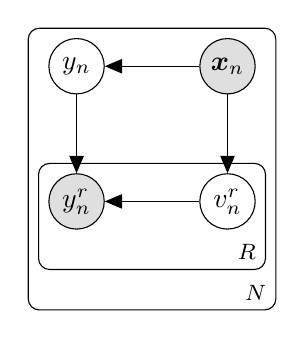
\begin{tikzpicture}

% Define nodes
\node[obs]                               (y) {$y_n^r$};
\node[latent, above=of y]                   (t) {$y_n$};
\node[obs, right=1.2cm of t]            (x) {$\ve{x}_n$};
\node[latent, right=1.2cm of y]            (v) {$v_{n}^r$};

% Connect the nodes
\edge {v,t} {y} ; %
\edge {x} {t,v} ; %

% Plates
\plate {ym} {(y)(v)} {$R$} ;
\plate {} {(x)(ym.north west)(ym.south east)} {$N$} ;

\end{tikzpicture}
%\endpgfgraphicnamed

%%% Local Variables: 
%%% mode: tex-pdf
%%% TeX-master: "example"
%%% End: 
}\hspace{0.5cm}
	\subfigure[\label{fig:GMb} Classification ]{% model_pca.tex
%
% Copyright (C) 2012 Jaakko Luttinen
%
% The MIT License
%
% See LICENSE file for more details.

% PCA model



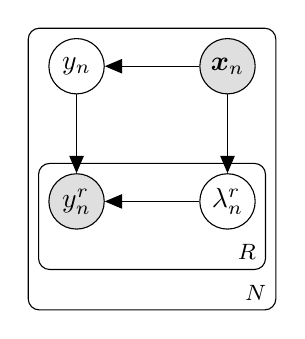
\begin{tikzpicture}

% Define nodes
\node[obs]                               (y) {$y_n^r$};
\node[latent, above=of y]                   (t) {$y_n$};
\node[obs, right=1.2cm of t]            (x) {$\ve{x}_n$};
\node[latent, right=1.2cm of y]            (v) {$\lambda_n^r$};

% Connect the nodes
\edge {v,t} {y} ; %
\edge {x} {t,v} ; %

% Plates
\plate {ym} {(y)(v)} {$R$} ;
\plate {} {(x)(ym.north west)(ym.south east)} {$N$} ;

\end{tikzpicture}
%\endpgfgraphicnamed

%%% Local Variables: 
%%% mode: tex-pdf
%%% TeX-master: "example"
%%% End: 
}
%	\label{fig:GM}
	\caption{Graphical plates for regression and classification models (see \cref{eq:RegLik} and \cref{eq:ClasLik}). Shaded nodes represent observed variables, and unshaded nodes indicate latent ones.}
	\label{fig:GM}
\end{figure}

%\begin{align}
%q(\ve{f}_j) = \int p(\ve{f}_j|\ve{u})q(\ve{u})d\ve{u}.
%\label{eq:Postf}
%\end{align}

%\begin{align}
%\label{eq:LowBound1}
%\mathcal{L}=&\sum_{n=1}^{N}\mathbb{E}_{\prod\limits^J_{j=1}q(f_j(\ve{x}_n))}\left[\log\left( p\left(\ve{y}_n|\bm{\theta}(\ve{x}_n)\right)\right)\right]-\cdots\nonumber\\
%&\cdots-\mathbb{D}_{KL}(q(\ve{u})||p(\ve{u}))\label{eq:LowBound2},
%\end{align}







\section{Experimental Set-up}\label{sec:expsetup}
\subsection{Datasets and simulated/provided annotations}\label{sec:datasets}
For both cases (regression and classification), we test our approaches CGPMA and CCGPMA using three types of datasets. Namely, \textit{fully synthetic data}, \textit{semi-synthetic data}, and \textit{fully real datasets}. 

\subsubsection{Regression}\label{sec:datasetsReg}
First, we generate \textit{fully synthetic data} as an one-dimensional regression problem, where the ground truth for the $n$-th sample correspond to $y_n = \sin(2\pi \boldx_n)\sin(6\pi \boldx_n)$, where the input matrix $\boldX$ is formed by randomly sampling 100 points in $[0,1]$ from a uniform distribution. Besides, the test instances are obtained by extracting equally spaced samples from the interval $[0,1]$.

Second, to control the label generation~\cite{ruiz2019learning}, we build \textit{semi-synthetic data} from six datasets devoted regression from the well-known {UCI repository}.~\footnote{http://archive.ics.uci.edu/ml}
The chosen datasets include: {Auto MPG Data Set}--(Auto), {Bike Sharing Dataset Data Set}--(Bike), {Concrete Compressive Strength Data Set}--(Concrete), {The Boston Housing Dataset}--(Housing),\footnote{See https://www.cs.toronto.edu/$\sim${d}elve/data/boston/bostonDetail.html for housing} {Yacht Hydrodynamics Data Set}--(Yacht), and {Relative location of CT slices on axial axis Data Set}--(CT).  

Third, we evaluate our proposal on one \textit{fully real dataset}, where both the input features and the annotations are captured from real-world problems. Namely, we use the music genre data, holding a collection of songs records labeled from one to ten depending on their music genre: classical, country, disco, hip-hop, jazz, rock, blues, reggae, pop, and metal. From this set, $700$ samples were published randomly in the AMT platform to obtain labels from multiples sources, 2946 labels were obtained from 44 workers; however, we only take into account the annotators who labeled at least 20\% of the available instances, thus, we use the information from $R = 7$ labelers. The feature extraction is performed by following the work by authors in \cite{rodrigues2013learning}, to obtain an input space with $P\igual124$. Note that initially, this dataset configures a problem of multiclass classification (with $10$ classes); however, in this experiment, we face it by using regression. \cref{tab:RegData} summarizes the tested datasets for the regression case.

\begin{table}[!tb]
	\caption{Datasets for regression.
	}
	\label{tab:RegData}
	\centering
	\resizebox{\linewidth}{!}{
		\begin{tabular}{ccccC{2cm}cC{2cm}}\toprule
			&& Name && Number of features && Number of instances\\\midrule
		\multirow{ 1}{*}{\textit{fully synthetic}}	&& synthetic && 1 && 100\\\midrule
		\multirow{ 6}{*}{\textit{semi-synthetic}}   && Auto&& 8 && 398\\ 
		                                            && Bike && 13 && 17389\\
		                                            && Concrete && 9 && 1030\\
		                                            && Housing && 13 && 506\\
		                                            && Yacht && 6 && 308\\
		                                            && CT && 384&&53500
		                                            \\\midrule
      	\multirow{ 1}{*}{\textit{fully real}}       && Music && 124 && 1000
      	\\\bottomrule
	\end{tabular}}
\end{table}


As we pointed out previously, \textit{fully synthetic} and \textit{semi-synthetic} datasets do not hold real annotations. Thus, it is necessary to generate these labels synthetically as a version of the gold standard corrupted by Gaussian noise, i.e., $y_n^r = y_n +\epsilon_{r,n}$, where $\epsilon_{r,n}\sim \gauss(0, v_{r,n})$, being the $r$-th annotator error-variance for the sample $n$. Note that we are interested in to model such error-variance for the $r$-th annotator $\boldv_{r}$ as a function of the input features, $h_r(\cdot):\mathcal{X}\to \Real^{+}$, which is correlated with the variances of the other labelers. For doing so, the error variances are generated as follows:
\begin{itemize}
    \item Define $Q$ functions $u_q(\cdot)$, and the combination parameters $w_{r,q},\,\forall r, n$.
    \item For each annotator $r$ and sample $n$, compute $f_{r,n} = \sum_{q=1}^{Q}w_{r,q}u_q(x_n)$, where $x_n$ is the $n$-th component of $\ve{x}\in \Real$, which is an $1-$D representation of input features $\mat{X}$ by using the t-distributed Stochastic Neighbor Embedding approach \cite{maaten2008visualizing}.
    \item Finally, determine $v_{r,n} = \exp(f_{r,n})$. 
\end{itemize}

\subsubsection{Classification}\label{sec:datasetsCla}
Alike to regression, we test our CGPMA and CCGPMA approaches in three kinds of datasets. First, we generate \textit{fully synthetic data} as one-dimensional multi-class classification problem (K=3). The input matrix $\boldX$ is formed by randomly sampling $N=100$ points in $[0,1]$ from a uniform distribution. The true label for the $n$-th input sample $\boldx_n$ is generated by taking $\arg \max (t_{1,n}, t_{2,n}, t_{3,n})$, where each value $t_{1,n}, t_{2,n}, t_{3,n}$ is respectively generated by evaluating $\boldx_n$ in the following functions $\sin(2\pi\boldx_n))$, $-\sin(2\pi\boldx_n))$, and $-\sin(2\pi(\boldx_n+0.25))+0.5$. Besides, the test instances are obtained by extracting $200$ equally spaced samples from the interval $[0,1]$.

Second, to control the label generation~\cite{ruiz2019learning}, we build \textit{semi-synthetic data} from seven datasets devoted to binary and multi class-classification of the well-known {UCI repository}~\footnote{http://archive.ics.uci.edu/ml}.
The chosen datasets include: {Wisconsin Breast Cancer Database}--(breast), {BUPA liver disorders}--(bupa), {Johns Hopkins University Ionosphere database}--(ionosphere), {Pima Indians Diabetes Database}--(pima), {Tic-Tac-Toe Endgame database}--(tic-tac-toe), {Wine Data set}--(Wine), and {Image Segmentation Data Set}--(Segmentation). Moreover, we use the publicly available bearing data collected by the Case Western Reserve University--(Western). The aim is to build a system to diagnose the status of an electric motor based on the information from two accelerometers. The feature extraction and selection stage was performed by following \cite{hernandez2020bearing}.

Third, we evaluate our proposal on two \textit{fully real datasets}, where both the input features and the annotations are captured from real-world problems. Namely, we use a biosignal database, where the goal is to build a system to evaluate the presence/absence of voice pathologies. In particular, a subset ($N\igual218$) of the Massachusetts Eye and Ear Infirmary Disordered Voice Database from the Kay Elemetrics company is utilized, which comprises voice records from healthy and different voice issues.  Each record is parametrized by the Mel-frequency cepstral coefficients (MFCC) to obtain an input space with $P\igual13$.  A set of physicians assess the voice quality by following the GRBAS protocol that comprises the evaluation of five qualitative scales: Grade of dysphonia--(G), Roughness--(R), Breathiness--(B), Asthenia--(A), and Strain--(S). For each perceptual scale, the specialist assigns a tag ranging from 0 (healthy voice) to 3 (severe disease)~\cite{arias2011automatic}. Accordingly, we face five multi-class classification problems (one per scale); however, we follow the procedure in~\cite{gil2018learning}, aiming to convert them into five binary classification problems due to the binary settings we have access to the ground truth~\cite{gonzalez2015automatic}. Further, the music genre data (used for the regression experiments) is also taken into account. We recall that such a dataset set configures a multi-class classification problem. \cref{tab:ClaData} summarizes the tested datasets for the regression case.

\begin{table}[!tb]
	\caption{Datasets used for classification.
	}
	\label{tab:ClaData}
	\centering
	\resizebox{\linewidth}{!}{
		\begin{tabular}{ccccC{2cm}cC{2cm}cC{2cm}}\toprule
			&& Name && Number of features && Number of instances && Number of classes\\\midrule
		\multirow{ 1}{*}{\textit{fully synthetic}}	&& synthetic && 1 && 100 && 3\\\midrule
		\multirow{ 8}{*}{\textit{semi-synthetic}}   && Breast&& 9 && 683 && 2\\ 
		                                            && Bupa && 6 && 345 && 2\\
		                                            && Ionosphere && 34 && 351 && 2\\
		                                            && Pima && 8 && 768 && 2\\
		                                            && Tic-tac-toe && 9 && 958 && 2\\
		                                            && Western && 7 && 3413 && 4\\
		                                            && Wine && 13 && 178 && 3\\
		                                            && Segmentation && 18 && 2310 && 7 \\\midrule
      	\multirow{ 2}{*}{\textit{fully real}}       && Voice && 13 && 218 && 2\\
      	                                            && Music && 124 && 1000 && 10\\\bottomrule
	\end{tabular}}
\end{table}

Similar to the regression case, \textit{fully synthetic} and \textit{semi-synthetic} datasets do not hold real annotations. Therefore, it is necessary to simulation those labels as corrupted versions of the hidden ground truth. Such simulation is performed by taking into account that there exist dependencies among the annotators and that the labelers' performance is a function of the input features. Accordingly, we simulate these labels as follows
\begin{itemize}
    \item Define $Q$ functions $u_q(\cdot)$, and the combination parameters $w_{r,q},\,\forall r, n$.
    \item For each annotator $r$ and sample $n$, compute $f_{r,n} = \sum_{q=1}^{Q}w_{r,q}u_q(x_n)$, where $x_n$ is the $n$-th component of $\ve{x}\in \Real$, which is an $1-$D representation of input features $\mat{X}$ by using the t-distributed Stochastic Neighbor Embedding approach \cite{maaten2008visualizing}.
    \item Determine $\lambda_{n}^r = \sigma(f_{r,n})$. 
    \item Finally, the label $y_n^r = \begin{cases}y_n, &\mbox{if }\lambda_{n}^r \ge 0.5\\ \tilde{y}_n, & \mbox{if }\lambda_{n}^r <0.5 \end{cases}$, where $\tilde{y}_n$ is the flipped version of the actual label $y_n$
\end{itemize}


\subsection{CGPMA and CCGPMA training}\label{sec:training}
Overall, the Radial basis function--(RBF) kernel is preferred in pattern classification because of its universal approximating ability and mathematical tractability. Hence, all the kernel functions for both CGPMA and CCGPMA are fixed as
\begin{align}\label{eq:RBF}
\kappa_j(\boldx_n, \boldx_{n^{\prime}})=\kappa_q(\boldx_n, \boldx_{n^{\prime}}) = \theta_1\exp\left(\frac{-\|\boldx_n- \boldx_{n^{\prime}} \|_2^2}{2\bm{\theta}_2^2}\right),
\end{align}
where $\|\cdot\|_2$ is the L$2$ norm, $n,n^{\prime} \in \left\{0,\dots , N\right\}$, and $\theta_1\in \Real$ and $\bm{\theta}_2\in (\Real^{+})^{P}$ ($\Real^{+}$ stands for the positive real numbers) are the kernel hiperparameters. For concrete testing we fix $\theta_1 = 1$, while $\bm{\theta}_2$ is estimated by optimizing the corresponding ELBO for CGPMA and CCGPMA. We emphasize that all GP-based approaches in this work are based on this type of kernel.\\
Another relevant parameter in the training of our CGPMA and CCGPMA is the number of required LFs. For CGPMA, it is clear that $Q$ have to be equal to the number of likelihood parameters $J$ since each function $f_j(\cdot)$ is linked to a LF $u_q(\cdot)$; accordingly, for regression, we fix $Q=R+1$, and $Q=R+K$, for classification scenarios. On the other hand, for CCGPMA, each $f_j(\cdot)$ is built as a convex combination of LFs $u_q(\cdot)$ (see \cref{eq:SLFM}), therefore, there is no any restriction about the number of $Q$. However, to make a fair comparison with CGPMA, we fix $Q=J$. Furthermore, for \textit{fully synthetic datasets}, we use $M=10$ inducing points per latent function, and for the remaining experiments, we test with $M=40$, and $M=80$. Finally, for all the experiments, we use stochastic inference with a mini-batch size of $100$.

\subsection{Method comparison and performance metrics}
\subsubsection{Regression}
\begin{table}[bt!]
	\caption{A brief overview of state-of-the-art methods tested for regression tasks. GPR: Gaussian Processes Regression, LR: logistic regression, Av: average, MA: multiple annotators, DL: Deep learning, LFCR: Learning from crowds for regression.
	}
	\label{tab:RegVal}
	\centering
	\resizebox{1\linewidth}{!}{
		\begin{tabular}{lcl}\toprule
			Algorithm && Description \\\midrule
			GPR-GOLD  && A GPR using the real labels (upper bound).\\
			GPR-Av    &&  A GPR using the average of the labels as the ground truth.\\
			MA-LFCR~\cite{raykar2010learning}  && A LR model for MA where the labelers' parameters\\
			&& are supposed to be constant across the input space.\\
			%MA-LMO~\cite{xiao2013learning}   && A multi-labeler approach where\\
			%&&the sources parameters depend on the input space.\\
			MA-GPR~\cite{rodrigues2014gaussian}	 &&  A multi-labeler GPR, which is as an extension of MA-LFCR.\\
			MA-DL~\cite{rodrigues2018deep}  && A Crowd Layer for DL, where the annotators' parameters\\
			&&  are constant across the input space.\\\bottomrule
	\end{tabular}}
\end{table}
The quality assessment is carried out by estimating the regression performance as the coefficient of determination--($R^2$). A cross-validation scheme is employed with 15 repetitions where $70$\% of the samples are utilized for training and the remaining $30\%$ for testing (except for \textit{fully synthetic dataset}, since it clearly defines the training and testing sets). \cref{tab:RegVal} displays the employed methods of the state-of-the-art for comparison purposes. From \cref{tab:RegVal}, we highlight that for the model MA-DL, the authors provided three different annotators' codification: MA-DL-B, where the bias for the annotators is measured; MA-DL-S, where the labelers' scale is computed; and measured; MA-DL-B+S, which is a version with both \cite{rodrigues2018deep}. Besides, it is worth clarifying that GPR-GOLD and GPR-Av are built from a sparse approximation based on inducing points (similar to the exposed in \cref{sec:CGP}) combined with stochastic variational inference; hence we use mini-batches with a size of $100$. Further, for the \textit{fully synthetic dataset} we fix $M=10$, and we tested with $M=40$, and $M=80$ for the rest of experiments.

\subsubsection{Classification}
The classification performance is assessed as the Area Under the Curve--(AUC). Further, the AUC is extended for multi-class settings, as discussed by authors in~\cite{fawcett2006introduction}. Similarly to the regression case, a cross-validation scheme is employed with 15 repetitions where $70$\% of the samples are utilized for training and the remaining $30\%$ for testing (except for music dataset, since its clearly define the training and testing sets). \cref{tab:ClaVal} displays the employed methods of the state-of-the-art for comparison purposes. 
\begin{table}[bt!]
	\caption{A brief overview of the state-of-the-art methods tested. GPC: Gaussian Processes classifier, LRC: logistic regression classifier, MV: majority voting, MA: multiple annotators, MAE: Modelling annotators expertise, LFC: Learning from crowds, DGRL: Distinguishing good from random labelers, KAAR: kernel alignment-based annotator relevance analysis.
	}
	\label{tab:ClaVal}
	\centering
	\resizebox{1\linewidth}{!}{
		\begin{tabular}{lcl}\toprule
			Algorithm && Description \\\midrule
			GPC-GOLD  && A GPC using the real labels (upper bound).\\
			GPC-MV    &&  A GPC using the MV of the labels as the ground truth.\\
			MA-LFC-C~\cite{raykar2010learning}  && A LRC with constant parameters across the input space.\\
			MA-DGRL~\cite{rodrigues2013learning}   && A multi-labeler approach that considers as latent variables\\ && the annotator performance.\\
            MA-GPC~\cite{rodrigues2014gaussian}	 &&  A multi-labeler GPC, which is as an extension of MA-LFC\\
            MA-GPCV~\cite{morales2019scalable} &&  An extension of MA-GPC, by using variational inference\\
            &&and including priors over the labelers' parameters.\\
            MA-DL~\cite{rodrigues2018deep}  && A Crowd Layer for DL, where the annotators' parameters\\
			&&  are constant across the input space\\
			KAAR~\cite{gil2018learning}  &&  A kernel-based approach that employs a convex combination\\ 
			 &&  of classifiers and codes labelers dependencies.\\\bottomrule
	\end{tabular}}
\end{table}

\section{Results and Discussion}
In this section, we expose the results regarding real-valued data (regression), and categorical data (classification), for the three types of cases that we have defined in previous section: \textit{fully synthetic data}, \textit{semi synthetic data}, and \textit{fully real data}.

\subsection{Regression}
\subsubsection{fully synthetic data}
We perform a controlled experiment aiming to verify the capability of our CGPMA and CCGPMA to estimate the performance of inconsistent annotators as a function of the input space and taking into account their dependencies. For this first experiment, we use the \textit{fully synthetic} dataset described in \cref{sec:datasetsReg}. We simulate five labelers ($R=5$) with different levels of expertise. To simulate the error-variances, we define $Q=3$ functions $u_q(\cdot)$, which are given as 
\begin{align}
\label{eq:u1r}
\notag u_1(x) &= 4.5\cos(2\pi x + 1.5\pi) - 3\sin(4.3\pi x + 0.3\pi) +\cdots\\ & \cdots + 4\cos(7\pi x + 2.4\pi),\\
\label{eq:u2r}
\notag u_2(x) &= 4.5\cos(1.5\pi x + 0.5\pi) + 5\sin(3\pi x + 1.5\pi) - \cdots\\ & \cdots - 4.5\cos(8\pi x+ 0.25\pi),\\
\label{eq:u3r}
u_3(x) &= 1,
\end{align}
where $x\in [0,1]$. Besides, we define the following combination matrix $\boldW \in \Real^{Q\times R}$, where
\begin{align}
\boldW=\begin{bmatrix}
-0.10  &  0.01   & -0.05 &  0.01  & -0.01\\
0.10   &  -0.01  & 0.01  &  -0.05 & 0.05\\
-2.3   &  -1.77  & 0.54  &  0.9   & 1.42
\end{bmatrix},
\label{eq:parametersP}
\end{align}
holding elements $w_{r,q}$.
% \begin{figure}[!bt]
% 	\centering
% 	%\begin{tikzpicture}[]
% 	    \begin{tikzpicture}[]
\begin{axis}[
width=0.45\textwidth,
xmin=0, xmax=1,
ymin=-8.5, ymax=11.5,
legend style={fill=white, fill opacity=1, draw opacity=1,text opacity=1},
xtick={0,0.2,0.4,0.6,0.8,1.0},
x tick label style={font=\footnotesize, align=center},
y tick label style={font=\footnotesize, align=center},
legend style={font=\small},
legend cell align={left},
cycle list name=color list,legend columns=-1,]
\addplot+[very thick,smooth]table{Figures/u0.dat};
\addlegendentry{$u_1(\cdot)$};
\addplot+[very thick,smooth]table{Figures/u1.dat};
\addlegendentry{$u_2(\cdot)$};
\addplot[very thick,green,domain=0:1]{1};
\addlegendentry{$u_3(\cdot)$};
\end{axis}
\end{tikzpicture}
% 	%\end{tikzpicture}
% 	\caption{Functions $u_q(\cdot)$ used to generate the error variances for regression experiments.}
% 	\label{fig:UqRegression}
% \end{figure}
\begin{figure*}[!tb]
	\centering
% 	\begin{tikzpicture}[]
\begin{axis}[scale=.6,name=plot1, xmin=0, xmax=1,ymin=-1.25,ymax=1.1,
x tick label style={font=\footnotesize, align=center},
y tick label style={font=\footnotesize, align=center},
legend style={font=\small},
legend cell align={left},
cycle list name=color list,ytick={-0.8,-0.4,0,0.4,0.8},
%ymajorgrids=true,xmajorgrids=true,grid style=dashed,
title={GPR-GOLD}]
\addplot+[opacity=1,dashed,thick,smooth,black]table{Figures/GT.dat};
\addplot+[opacity=1,blue,very thick,smooth]table{Figures/GPGT.dat};
\addplot+[opacity=0,name path=A,very thick,smooth,red]table{Figures/GPGTU.dat};
\addplot+[opacity=0,name path=B,very thick,smooth,red]table{Figures/GPGTL.dat};
\addplot[opacity=0.3,blue!50] fill between[of=A and B];
\end{axis}
\begin{axis}[scale=.6,name=plot2,at={($(plot1.north east)+(0.12cm,0cm)$)},anchor=north west, xmin=0, xmax=1,ymin=-1.25,ymax=1.1,x tick label style={font=\footnotesize, align=center},
y tick label style={font=\footnotesize, align=center},legend style={font=\small},
legend cell align={left},cycle list name=color list,yticklabel=\empty,xticklabel=\empty, %xticklabel=\empty,ytick={-0.8,-0.4,0,0.4,0.8},ymajorgrids=true,xmajorgrids=true,grid style=dashed,
title={GPR-Av}]
\addplot+[opacity=1,dashed,thick,smooth,black]table{Figures/GT.dat};
\addplot+[opacity=1,blue,very thick,smooth]table{Figures/GPAv.dat};
\addplot+[opacity=0,name path=A,very thick,smooth,red]table{Figures/GPAvU.dat};
\addplot+[opacity=0,name path=B,very thick,smooth,red]table{Figures/GPAvL.dat};
\addplot[opacity=0.3,blue!50] fill between[of=A and B];
\end{axis}
\begin{axis}[scale=.6,name=plot3,at={($(plot2.north east)+(0.12cm,0cm)$)},anchor=north west, xmin=0, xmax=1,ymin=-1.25,ymax=1.1,x tick label style={font=\footnotesize, align=center},
y tick label style={font=\footnotesize, align=center},legend style={font=\small},
legend cell align={left},cycle list name=color list,yticklabel=\empty,xticklabel=\empty, %xticklabel=\empty,ytick={-0.8,-0.4,0,0.4,0.8},ymajorgrids=true,xmajorgrids=true,grid style=dashed,
title={MA-LFCR}]
\addplot+[opacity=1,dashed,thick,smooth,black]table{Figures/GT.dat};
\addplot+[opacity=1,blue,very thick,smooth]table{Figures/LFCR.dat};
\end{axis}
\begin{axis}[scale=.6,name=plot4,at={($(plot3.north east)+(0.12cm,0cm)$)},anchor=north west, xmin=0, xmax=1,ymin=-1.25,ymax=1.1,x tick label style={font=\footnotesize, align=center},
y tick label style={font=\footnotesize, align=center},legend style={font=\small},
legend cell align={left},cycle list name=color list,yticklabel=\empty,xticklabel=\empty, %xticklabel=\empty,ytick={-0.8,-0.4,0,0.4,0.8},ymajorgrids=true,xmajorgrids=true,grid style=dashed,
title={MA-GPR}]
\addplot+[opacity=1,dashed,thick,smooth,black]table{Figures/GT.dat};
\addplot+[opacity=1,blue,very thick,smooth]table{Figures/GPM.dat};
\addplot+[opacity=0,name path=A,very thick,smooth,red]table{Figures/GPU.dat};
\addplot+[opacity=0,name path=B,very thick,smooth,red]table{Figures/GPL.dat};
\addplot[opacity=0.3,blue!50] fill between[of=A and B];
\end{axis}
\begin{axis}[scale=.6,name=plot5,at={($(plot2.south west)+(0cm,-1.0cm)$)},anchor=north west, xmin=0, xmax=1,ymin=-1.25,ymax=1.1,x tick label style={font=\footnotesize, align=center},
y tick label style={font=\footnotesize, align=center},legend style={font=\small},
legend cell align={left},cycle list name=color list,yticklabel=\empty,xticklabel=\empty, %xticklabel=\empty,ytick={-0.8,-0.4,0,0.4,0.8},ymajorgrids=true,xmajorgrids=true,grid style=dashed,
title={MA-DL},cycle list name=color list,legend columns=-1,legend style={fill=white, fill opacity=1, draw opacity=1,text opacity=1},legend style={font=\footnotesize},]
\addplot+[forget plot,opacity=1,dashed,thick,smooth,black]table{Figures/GT.dat};
\addplot+[opacity=1,very thick,smooth,blue]table{Figures/MADLB.dat};
\addlegendentry{B};
\addplot+[opacity=1,very thick,smooth,red]table{Figures/MADLS.dat};
\addlegendentry{S};
\addplot+[opacity=1,very thick,smooth,green]table{Figures/MADLB+S.dat};
\addlegendentry{B+S};
\end{axis}
\begin{axis}[scale=.6,name=plot6,at={($(plot5.north east)+(0.12cm,0cm)$)},anchor=north west, xmin=0, xmax=1,ymin=-1.25,ymax=1.1,x tick label style={font=\footnotesize, align=center},
y tick label style={font=\footnotesize, align=center},legend style={font=\small},
legend cell align={left},cycle list name=color list,yticklabel=\empty, %xticklabel=\empty,ytick={-0.8,-0.4,0,0.4,0.8},ymajorgrids=true,xmajorgrids=true,grid style=dashed,
title={CGPMA-R},xticklabel=\empty,]
\addplot+[opacity=1,dashed,thick,smooth,black]table{Figures/GT.dat};
\addplot+[opacity=1,blue,very thick,smooth]table{Figures/CGPM.dat};
\addplot+[opacity=0,name path=A,very thick,smooth,red]table{Figures/CGPU.dat};
\addplot+[opacity=0,name path=B,very thick,smooth,red]table{Figures/CGPL.dat};
\addplot[opacity=0.3,blue!50] fill between[of=A and B];
\end{axis}
\begin{axis}[scale=.6,name=plot7,at={($(plot6.north east)+(0.12cm,0cm)$)},anchor=north west, xmin=0, xmax=1,ymin=-1.25,ymax=1.1,x tick label style={font=\footnotesize, align=center},
y tick label style={font=\footnotesize, align=center},legend style={font=\small},
legend cell align={left},cycle list name=color list,yticklabel=\empty, xticklabel=\empty,
%ytick={-0.8,-0.4,0,0.4,0.8},ymajorgrids=true,xmajorgrids=true,grid style=dashed,
title={CCGPMA-R}]
\addplot+[opacity=1,dashed,thick,smooth,black]table{Figures/GT.dat};
\addplot+[opacity=1,blue,very thick,smooth]table{Figures/CCGPM.dat};
\addplot+[opacity=0,name path=C,very thick,smooth,blue]table{Figures/CCGPU.dat};
\addplot+[opacity=0,name path=D,very thick,smooth,blue]table{Figures/CCGPL.dat};
\addplot[opacity=0.3,blue!50] fill between[of=C and D];
\end{axis}
\end{tikzpicture}
	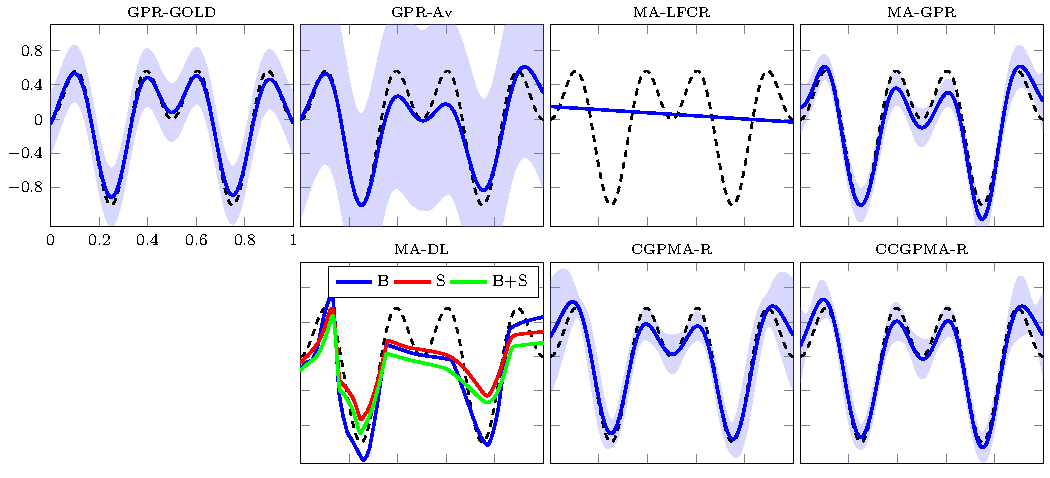
\includegraphics[width = \textwidth]{Figures/SinReg.pdf}
	\caption{Fully synthetic dataset results. We compare the prediction of our CCGPMA-R($R^2=0.9438$), and CCGPMA-R($R^2=0.9280$) with the theoretical upper bound GPR-GOLD($R^2=0.9843$) and lower bound GPR-Av($R^2=0.8718$), and state-of-the-art approaches, MA-LFCR($R^2=-0.0245$), MA-GPR($R^2=0.9208$),  MA-DL-B($R^2=0.7020$), MA-DL-S($R^2=0.6559$), MA-DL-B+S($R^2=0.5997$). Note that we provided the Gold Standard in dashed lines. The shaded region in GPR-Av, MA-GPR, CGPMA-R, and CCGPMA-R indicates the area enclosed by the mean plus or minus two standard deviations. We remark that there is no shaded region for MA-LFCR, and DLMA since these approaches do not provide information about the prediction uncertainty.}
	\label{fig:FSReg}
\end{figure*}
\cref{fig:FSReg} shows the predictive performance of all methods in this first experiment. The results show two clear groups: those based on GPs (GPR-Av, MA-GPR, CGPMA-R, and CCGPMA-R), which expose the best performance in terms of the $R^2$ score, and those based on other types of approaches (MA-LFCR, and MA-DL), whose performance is not satisfactory. The behavior of MA-LFCR is not unexpected since it only can deal with linear problems. Besides, concerning MA-DL and its three variations (S, B, and S+B), we note that this approach, in general terms, has the capability of modeling the non-linearities present in the regression problem; however, MA-DL exposes a significant low performance (even lower than the most naive approach, GPR-Av), which is a bit surprising due to the DL models have shown significant advances in the artificial intelligence context \cite{schmidhuber2015deep}. Such an outcome is explained because these crowd layers provide a very simple codification of the annotators' performance to guarantee a low computational cost \cite{morales2019scalable1}; therefore, MA-DL does not provide a proper codification of the annotators' behavior. \\
Among the GP-based methods, the proposed CCGPMA-R exposes the best result, followed closely by our CGPMA-R and MA-GPR. Notice that the performance of GPR-Av is also close to them, which indicates that this experiment seems not to be too challenging for the GPs-based approaches; nevertheless, notorious differences will be appreciated in the next experiments.

On the other hand, concerning the significant high performance of our CCGPMA-R (the best in terms of $R^2$ score), we hypothesize that such an outcome is a consequence that our approach offers a better representation of the labelers' behavior when compared with its competitors. To empirically support the above hypothesis, \cref{fig:ExpReg} shows the estimated error-variances for this first experiment; here, we only take into account the models that include these parameters in their formulations. From \cref{fig:ExpReg}, we note from the $R^2$ score and making a visual inspection that the approaches MA-LFCR and MA-GPR (see columns 2 and 3 in \cref{fig:ExpReg}) offer the worst representation for the annotator's performance, which is expected due to such models do not take into account the relationship between the annotators' performance and the input space. Conversely, our CGPMA-R and CCGPMA-R (see columns 4 and 5 in \cref{fig:ExpReg}) clearly outperforms the models named previously. This outcome is a consequence that our two approaches compute such error-variances as functions of the input features, allowing for a better codification of the labelers' behavior. Besides, by making a visual inspection and analyzing the $R^2$ scores, CCGPMA-R performs better that CGPMA-R; in principle, this is a bit unexpected since both approaches compute the labelers' parameters as non-linear functions; however, we highlight that contrary to CGPMA-R, CCGPMA-R models the annotators' interdependencies, which improves the modeling of such performances as was empirically demonstrated in \cite{zhu2019unsupervised}. Finally, we remark that although our CCGPMA-R offers the best representation of the annotators' performance, the results for Annotators 2 and 3 (rows 2 and 3 in the fifth column of \cref{fig:ExpReg}) seem to be unsatisfactory. Such an outcome is caused by the quasi-periodic behavior in the error-variances for those labelers, which cannot be captured by our approach because we are using a kernel RBF, as we pointed out in \cref{sec:training}.

\begin{figure*}[!tb]
	\centering
	%\input{Figures/VarEXp.tex}
	\includegraphics[width = \textwidth]{Figures/VarEXp.pdf}
	\caption{Estimated values of error-variance for the five annotators in the \textit{fully synthetic} experiment. In the first column, from top to bottom, we expose the error-variances $\boldv_r$ used to simulate the labels from each annotator. Furthermore, the subsequent columns from top to bottom present the estimation of such error-variances performed by state-of-the-art models that include these kinds of parameters in their formulation; moreover, the true error-variances are provided in dashed lines. The shaded region in CGPMA-R and CCGPMA-R indicates the area enclosed by the mean plus or minus two standard deviations. We remark that there is no shaded region for MA-LFCR, and MA-GPR since these approaches perform a fixed-point estimation for the annotators' parameters. Finally, we remark that the $R^2$ score between the true and estimated error variances are provided.}
	\label{fig:ExpReg}
\end{figure*}

\subsubsection{Semi-synthetic data results}
\begin{table*}[!htb]
	\centering
	%\tiny
	\scriptsize 
	\caption{Regression results in terms of $R^2$ score over \textit{semi synthetic datasets}. Bold: the highest $R^2$ excluding the upper bound GPR-GOLD.}
	\resizebox{.98\linewidth}{!}{
	\begin{tabular}{cccccccc}\toprule
		{Method} & {Auto} & {Bike} & {Concrete} & {Housing} & {Yacht} & {CT} & {Average}\\\midrule
		GPR-GOLD($M=40$)&$0.8604\pm0.0271$ & $0.5529\pm0.0065$ & $0.8037\pm0.0254$ & $0.8235\pm0.0419$ & $0.8354\pm0.0412$ & $0.8569\pm0.0055$ & $0.7888$\\ 
        GPR-GOLD($M=80$)&$0.8612\pm0.0279$ & $0.5603\pm0.0063$ & $0.8271\pm0.0230$ & $0.8275\pm0.0399$ & $0.8087\pm0.0423$ & $0.8648\pm0.0047$ & $0.7916$\\ 
        GPR-Av($M=40$)  &$0.8425\pm0.0286$ & $0.5280\pm0.0100$ & $0.7589\pm0.0279$ & $0.7834\pm0.0463$ & $0.7588\pm0.0498$ & $0.8070\pm0.0130$ & $0.7464$\\ 
        GPR-Av($M=80$)  &$0.8406\pm0.0304$ & $0.5397\pm0.0085$ & $0.7765\pm0.0274$ & $0.7903\pm0.0451$ & $0.7676\pm0.0535$ & $0.8167\pm0.0089$ & $0.7552$\\ 
        MA-LFCR         &$0.7973\pm0.0218$ & $0.3385\pm0.0051$ & $0.6064\pm0.0384$ & $0.7122\pm0.0509$ & $0.6403\pm0.0186$ & $\mathbf{0.8400\pm0.0014}$ & $0.6558$\\ 
        MA-GPR          &$0.8456\pm0.0281$ & $0.4448\pm0.0187$ & $0.7769\pm0.0367$ & $0.7685\pm0.0632$ & $0.7842\pm0.1027$ & $0.0105\pm0.0045$ & $0.6051$\\
        MA-DL-B         &$0.7766\pm0.0253$ & $0.5854\pm0.0107$ & $0.2319\pm0.0328$ & $0.5317\pm0.1005$ & $0.2089\pm0.0783$ & $0.6903\pm0.2689$ & $0.5041$\\ 
        MA-DL-S         &$0.7761\pm0.0279$ & $\mathbf{0.5828\pm0.0149}$ & $0.2363\pm0.0252$ & $0.5352\pm0.0948$ & $0.1822\pm0.0985$ & $0.9394\pm0.0257$ & $0.5420$\\ 
        MA-DL-B+S       &$0.7717\pm0.0239$ & $0.5816\pm0.0181$ & $0.2369\pm0.0322$ & $0.5330\pm0.0850$ & $0.1974\pm0.0895$ & $0.5517\pm0.2316$ & $0.4787$\\ 
        CGPMA-R($M=40$) &$0.8474\pm0.0221$ & $0.5464\pm0.0069$ & $0.8169\pm0.0231$ & $0.7946\pm0.0498$ & $0.7545\pm0.1029$ & $0.8236\pm0.0132$ & $0.7639$\\ 
        CGPMA-R($M=80$) &$0.7768\pm0.0708$ & $0.5560\pm0.0074$ & $0.8190\pm0.0254$ & $0.8058\pm0.0493$ & $0.8230\pm0.0760$ & $0.8371\pm0.0104$ & $0.7696$\\ 
        CCGPMA-R($M=40$)&$0.8563\pm0.0247$ & $0.5284\pm0.0117$ & $0.7976\pm0.0270$ & $0.7994\pm0.0462$ & $0.8436\pm0.0507$ & $0.8219\pm0.0062$ & $0.7745$\\ 
        CCGPMA-R($M=80$)&$\mathbf{0.8578\pm0.0244}$ & $0.5467\pm0.0069$ & $\mathbf{0.8220\pm0.0259}$ & $\mathbf{0.8110\pm0.0453}$ & $\mathbf{0.8476\pm0.0544}$ & $0.8252\pm0.0083$ & $\mathbf{0.7850}$\\\bottomrule
	\end{tabular}}
	\label{tab:SSRegResults}
\end{table*}
as for the \textit{fully synthetic data} (see \cref{eq:u1r,eq:u2r,eq:u3r,eq:parametersP}). \cref{tab:SSRegResults} shows the results for this second experiment with \textit{semi synthetic dataset}. On average, our CCGPMA-R  exhibits the best generalization performance in terms of the $R^2$ score. Besides, regarding its GPs-based competitors (GPR-Av, MA-GPR, and CGPMA-R), we first note that the performance of our CGPMA-R is a bit lower than CCGPMA-R. The above is not an unexpected outcome since both approaches estimate the annotators' performances as functions of the input features, which fixes the process that we use to simulate the labels for this experiment (see \cref{sec: datasets}). Secondly, as expected, the intuitive lower bound GPR-Av exhibits a significantly worse prediction than our approaches. On the other hand, the behavior of MA-GPR is surprising due to it exhibits the most deficient prediction capability, even far worse than the supposed lower bound GPR-Av. The key to this abnormal behavior lies in the formulation of this approach; MA-GPR is based on a basic Gaussian process (i.e., without considering sparse approximations neither stochastic variational inference) that cannot handle large datasets. In fact, we note that MA-GPR exhibits the worst performances for datasets Bike, Concrete, and CT, which are conformed by a large number of samples (Respectively 17389, 1030, and 53500).
Next, we analyze the results concerning the linear model MA-LFR; attained to the results, we note that this approach's prediction capacity is not satisfactory since its performance is far lower than our approaches; the above outcome suggests that there may exist a non-linear structure in most databases. However, we highlight a particular result for the dataset CT, where MA-LFCR exhibits the best performance defeating all its competitors based on non-linear models. From the above, we intuit that the CT dataset may have a linear structure. To confirm this supposition, we perform an additional experiment over CT by training a regression scheme based on LR with the actual labels (we follow the same scheme as for GPR-GOLD). We obtain an $R^2$ score equal to $0.8541$ (on average), which is close to the results obtained by GPR-GOLD. Thus, we can elucidate that there exists a linear structure in the dataset CT. Hence, considering linear datasets, MA-LFR sets an attractive option. Finally, we analyze the results for the DL-based models. Similar to the experiments over \textit{fully synthetic datasets}, we note a considerable low prediction capacity; in fact, they are even defeated by the linear model MA-LFR Again, we attribute this behavior to the fact that the CrowdLayer (used to manage the data from multiple annotators) does not offer a suitable codification of the labelers' behavior. Nevertheless, taking the above into account, we observe an unusual result in the dataset Bike, where the DL-based approaches offer the best performance, even defeating the supposed upper-bound GPR-GOLD. To explain that, it is necessary to analyze the meaning of the target variable in such a dataset.  Attained to the description of this dataset,\footnote{Such description can be found in https://archive.ics.uci.edu/ml/datasets/bike+sharing+dataset} the target variables indicates the count of total rental bikes, including both casual and registered in a day. The above suggests that there may exist a quasi-periodic structure in the dataset, which cannot be captured by the GPR-GOLD since it uses a non-periodic kernel (it uses the RBF kernel). To support our suppositions, an additional experiment was performed over this dataset by training the model GPR-GOLD with the kernel defined as follows. 
\begin{align}\label{eq:Pkernel}
\kappa(\boldx_n, \boldx_{n^{\prime}}) = \varphi \exp \left[  - \frac{1}{2}\sum_{p=1}^{P}\left( \frac{\sin(\frac{\pi}{T_p} (x_{p,n}- x_{p,n^{\prime}}) )}{l_p}\right)^2 \right],
\end{align}
where $\varphi\in \Real$ is the variance parameter, $l_p\in (\Real^{+})$ is the length-scale parameter for the $p$-th dimension, and $T_p\in (\Real^{+})$ is the period for the $p$-th dimension. Therefore, we obtain an $R^2$ score equal to $0.5952$ (on average), which is greater than the obtained by the DL-based approaches, indicating a quasi-periodic structure in the Bike dataset as we had supposed.

\subsubsection{fully real data}
Until now, we have empirically demonstrated that our approaches CGPMA and CCGPMA offer a better representation of the labelers' behavior. Nevertheless, the previous experiments configure a controlled scenario due to the labels were simulated; hence, these results could be biased by the simulation method. In this sense, the \textit{fully real datasets} present the most challenging scenario, where both the input samples and the labels come from real-world applications. 
\begin{table}[!htb]
	\centering
	%\tiny
	\scriptsize 
	\caption{Regression results in terms of $R^2$ score over \textit{fully real dataset}. Bold: the highest $R^2$ excluding the upper bound GPR-GOLD.}
	\resizebox{.5\linewidth}{!}{
	\begin{tabular}{cc}\toprule
		{Method} & {Music}\\\midrule
		GPR-GOLD($M=40$)&$0.4704$\\
        GPR-GOLD($M=80$)&$0.4889$\\
        GPR-Av($M=40$)  &$0.2572$\\
        GPR-Av($M=80$)  &$0.2744$\\
        MA-LFCR         &$0.1404$\\
        MA-GPR          &$0.0090$\\
        MA-DL-B         &$0.2339$\\
        MA-DL-S         &$0.2934$\\
        MA-DL-B+S       &$0.3519$\\
        CGPMA-R($M=40$) &$0.3345$\\
        CGPMA-R($M=80$) &$0.3531$\\
        CCGPMA-R($M=40$)&$0.3337$\\
        CCGPMA-R($M=80$)&$\mathbf{0.3872}$\\\bottomrule
	\end{tabular}}
	\label{tab:FSRegResults}
\end{table}
\cref{tab:FSRegResults} outlines the achieved performances. We remark that our CCGPMA-R with $M=80$ obtains the best generalization performance in terms of $R^2$ score. Further, as theoretically expected, its performance lies between that of GPR-GOLD and GP-Av. 
Moreover, regarding the GPs-based competitors (MA-GPR and CGPMA-R), we note that similarly to previous experiments, our CGPMA-R is just a bit lower than CCGPMA-R, which is expected behavior due to both frameworks estimate the annotators' performances as functions of the input features. On the other hand, the behavior of MA-GPR is again surprising, due to it exhibits a prediction capability worse than GPR-Av. We remark that this outcome is due to over-fitting; in fact, the training $R^2$ score for MA-GPR is $0.4731$, which is comparable with GPR-GOLD. The linear approach MA-LFCR exhibits the second-lowest performance and performs worse than the theoretical lower bound GP-Av, which indicates a non-linear structure in the Music dataset. Finally, analyzing the results from the deep learning approaches, we note that the variation MA-DL-B+S exhibit performance similar to our CGPMA-R; however, it is a bit lower than our CCGPMA-R. We highlight that despite the capacities of deep learning, our approach CCGPMA-R offers a better representation of annotators' behavior, unlike the deep learning approaches, which measure such performance using a single parameter.\\
On the other hand, we observe that all regression models exposed a lower generalization performance than previous results (see \cref{tab:SSRegResults}), which is a repercussion of solving a multi-class classification problem with regression models. Such an outcome is not uncommon due to similar results are exposed in \cite{rodrigues2017learning,rodrigues2018deep}, where they used regression approaches to solve a multi-class classification problem. 

\subsection{Classification}
\subsubsection{Fully synthetic data} Alike the regression case, we first perform a controlled experiment to verify the capability of our CGPMA and CCGPMA with binary and multi-class classification with multiple annotators. For this first experiment, we use the \textit{fully synthetic} dataset described in \cref{sec:datasetsCla}. We simulate five labelers ($R=5$) with different levels of expertise. To simulate the error-variances, we define $Q=3$ functions $u_q(\cdot)$, which are given as 
\begin{align}
\label{eq:u1c}
u_1(x) &= 4.5\cos(2\pi x + 1.5\pi) - 3\sin(4.3\pi x + 0.3\pi),\\
\label{eq:u2c}
u_2(x) &= 4.5\cos(1.5\pi x + 0.5\pi) + 5\sin(3\pi x + 1.5\pi),\\
\label{eq:u3c}
u_3(x) &= 1,
\end{align}
where $x\in [0,1]$. Besides, we define the combination matrix $\boldW \in \Real^{Q\times R}$
\begin{figure*}[!tb]
	\centering
% 	\begin{tikzpicture}[]
\begin{axis}[scale=.6,name=plot1, xmin=0, xmax=1,ymin=-1.25,ymax=1.1,
x tick label style={font=\footnotesize, align=center},
y tick label style={font=\footnotesize, align=center},
legend style={font=\small},
legend cell align={left},
cycle list name=color list,ytick={-0.8,-0.4,0,0.4,0.8},
%ymajorgrids=true,xmajorgrids=true,grid style=dashed,
title={GPR-GOLD}]
\addplot+[opacity=1,dashed,thick,smooth,black]table{Figures/GT.dat};
\addplot+[opacity=1,blue,very thick,smooth]table{Figures/GPGT.dat};
\addplot+[opacity=0,name path=A,very thick,smooth,red]table{Figures/GPGTU.dat};
\addplot+[opacity=0,name path=B,very thick,smooth,red]table{Figures/GPGTL.dat};
\addplot[opacity=0.3,blue!50] fill between[of=A and B];
\end{axis}
\begin{axis}[scale=.6,name=plot2,at={($(plot1.north east)+(0.12cm,0cm)$)},anchor=north west, xmin=0, xmax=1,ymin=-1.25,ymax=1.1,x tick label style={font=\footnotesize, align=center},
y tick label style={font=\footnotesize, align=center},legend style={font=\small},
legend cell align={left},cycle list name=color list,yticklabel=\empty,xticklabel=\empty, %xticklabel=\empty,ytick={-0.8,-0.4,0,0.4,0.8},ymajorgrids=true,xmajorgrids=true,grid style=dashed,
title={GPR-Av}]
\addplot+[opacity=1,dashed,thick,smooth,black]table{Figures/GT.dat};
\addplot+[opacity=1,blue,very thick,smooth]table{Figures/GPAv.dat};
\addplot+[opacity=0,name path=A,very thick,smooth,red]table{Figures/GPAvU.dat};
\addplot+[opacity=0,name path=B,very thick,smooth,red]table{Figures/GPAvL.dat};
\addplot[opacity=0.3,blue!50] fill between[of=A and B];
\end{axis}
\begin{axis}[scale=.6,name=plot3,at={($(plot2.north east)+(0.12cm,0cm)$)},anchor=north west, xmin=0, xmax=1,ymin=-1.25,ymax=1.1,x tick label style={font=\footnotesize, align=center},
y tick label style={font=\footnotesize, align=center},legend style={font=\small},
legend cell align={left},cycle list name=color list,yticklabel=\empty,xticklabel=\empty, %xticklabel=\empty,ytick={-0.8,-0.4,0,0.4,0.8},ymajorgrids=true,xmajorgrids=true,grid style=dashed,
title={MA-LFCR}]
\addplot+[opacity=1,dashed,thick,smooth,black]table{Figures/GT.dat};
\addplot+[opacity=1,blue,very thick,smooth]table{Figures/LFCR.dat};
\end{axis}
\begin{axis}[scale=.6,name=plot4,at={($(plot3.north east)+(0.12cm,0cm)$)},anchor=north west, xmin=0, xmax=1,ymin=-1.25,ymax=1.1,x tick label style={font=\footnotesize, align=center},
y tick label style={font=\footnotesize, align=center},legend style={font=\small},
legend cell align={left},cycle list name=color list,yticklabel=\empty,xticklabel=\empty, %xticklabel=\empty,ytick={-0.8,-0.4,0,0.4,0.8},ymajorgrids=true,xmajorgrids=true,grid style=dashed,
title={MA-GPR}]
\addplot+[opacity=1,dashed,thick,smooth,black]table{Figures/GT.dat};
\addplot+[opacity=1,blue,very thick,smooth]table{Figures/GPM.dat};
\addplot+[opacity=0,name path=A,very thick,smooth,red]table{Figures/GPU.dat};
\addplot+[opacity=0,name path=B,very thick,smooth,red]table{Figures/GPL.dat};
\addplot[opacity=0.3,blue!50] fill between[of=A and B];
\end{axis}
\begin{axis}[scale=.6,name=plot5,at={($(plot2.south west)+(0cm,-1.0cm)$)},anchor=north west, xmin=0, xmax=1,ymin=-1.25,ymax=1.1,x tick label style={font=\footnotesize, align=center},
y tick label style={font=\footnotesize, align=center},legend style={font=\small},
legend cell align={left},cycle list name=color list,yticklabel=\empty,xticklabel=\empty, %xticklabel=\empty,ytick={-0.8,-0.4,0,0.4,0.8},ymajorgrids=true,xmajorgrids=true,grid style=dashed,
title={MA-DL},cycle list name=color list,legend columns=-1,legend style={fill=white, fill opacity=1, draw opacity=1,text opacity=1},legend style={font=\footnotesize},]
\addplot+[forget plot,opacity=1,dashed,thick,smooth,black]table{Figures/GT.dat};
\addplot+[opacity=1,very thick,smooth,blue]table{Figures/MADLB.dat};
\addlegendentry{B};
\addplot+[opacity=1,very thick,smooth,red]table{Figures/MADLS.dat};
\addlegendentry{S};
\addplot+[opacity=1,very thick,smooth,green]table{Figures/MADLB+S.dat};
\addlegendentry{B+S};
\end{axis}
\begin{axis}[scale=.6,name=plot6,at={($(plot5.north east)+(0.12cm,0cm)$)},anchor=north west, xmin=0, xmax=1,ymin=-1.25,ymax=1.1,x tick label style={font=\footnotesize, align=center},
y tick label style={font=\footnotesize, align=center},legend style={font=\small},
legend cell align={left},cycle list name=color list,yticklabel=\empty, %xticklabel=\empty,ytick={-0.8,-0.4,0,0.4,0.8},ymajorgrids=true,xmajorgrids=true,grid style=dashed,
title={CGPMA-R},xticklabel=\empty,]
\addplot+[opacity=1,dashed,thick,smooth,black]table{Figures/GT.dat};
\addplot+[opacity=1,blue,very thick,smooth]table{Figures/CGPM.dat};
\addplot+[opacity=0,name path=A,very thick,smooth,red]table{Figures/CGPU.dat};
\addplot+[opacity=0,name path=B,very thick,smooth,red]table{Figures/CGPL.dat};
\addplot[opacity=0.3,blue!50] fill between[of=A and B];
\end{axis}
\begin{axis}[scale=.6,name=plot7,at={($(plot6.north east)+(0.12cm,0cm)$)},anchor=north west, xmin=0, xmax=1,ymin=-1.25,ymax=1.1,x tick label style={font=\footnotesize, align=center},
y tick label style={font=\footnotesize, align=center},legend style={font=\small},
legend cell align={left},cycle list name=color list,yticklabel=\empty, xticklabel=\empty,
%ytick={-0.8,-0.4,0,0.4,0.8},ymajorgrids=true,xmajorgrids=true,grid style=dashed,
title={CCGPMA-R}]
\addplot+[opacity=1,dashed,thick,smooth,black]table{Figures/GT.dat};
\addplot+[opacity=1,blue,very thick,smooth]table{Figures/CCGPM.dat};
\addplot+[opacity=0,name path=C,very thick,smooth,blue]table{Figures/CCGPU.dat};
\addplot+[opacity=0,name path=D,very thick,smooth,blue]table{Figures/CCGPL.dat};
\addplot[opacity=0.3,blue!50] fill between[of=C and D];
\end{axis}
\end{tikzpicture}
	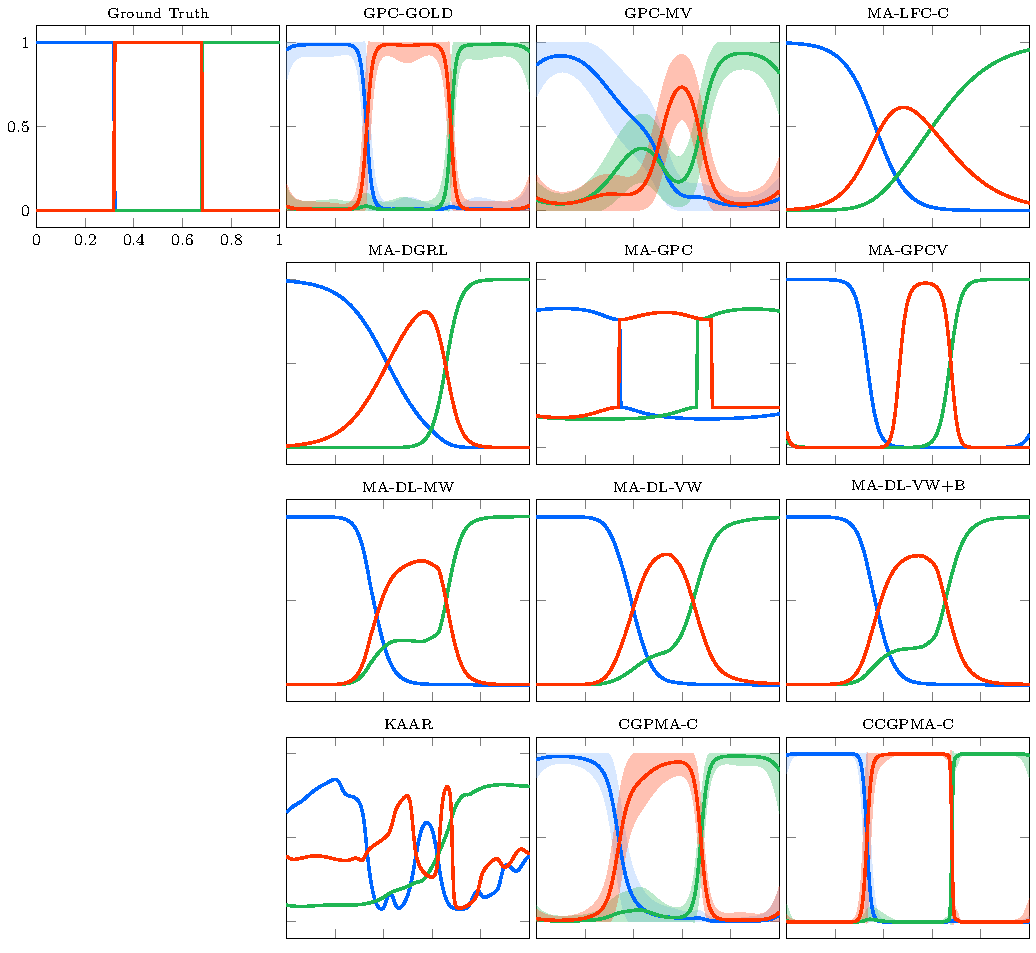
\includegraphics[width = \textwidth]{Figures/SinCla.pdf}
	\caption{Fully synthetic dataset results (blue=class 1, red=class 2, and green=class3). We compare the prediction of our CCGPMA-C($AUC=1$), and CCGPMA-C($AUC=0.9999$) with the theoretical upper bound GPC-GOLD($AUC=1.0$) and lower bound GPC-MV($AUC=0.9809$), and state-of-the-art approaches, MA-LFC-C($AUC=0.9993$), MA-DGRL($AUC=0.9999$),  MA-GPC($AUC=0.9977$), MA-GPCV($AUC=0.9515$), MA-DL-MW($AUC=0.9989$), MA-DL-VW($AUC=0.9972$), MA-DL-VW+B($AUC=0.9994$), KAAR($0.9099$). Note that the shaded region in GPC-MV, CGPMA-C, and CCGPMA-C indicates the area enclosed by the mean plus or minus two standard deviations. We remark that there is no shaded region for the rest of approaches since they do not provide information about the prediction uncertainty.}
	\label{fig:FSCla}
\end{figure*}
\begin{align}
\boldW=\begin{bmatrix}
0.4  &  0.7   & -0.5 &  0.0  & -0.7\\
0.4   &  -1.0  & -0.1  &  -0.8 & 1.0\\
3.1   &  -1.8  & -0.6  &  -1.2   & 1.0
\end{bmatrix},
\label{eq:parametersPC}
\end{align}
holding elements $w_{r,q}$. \cref{fig:FSCla} exposes the predictive performance for all approaches for the \textit{fully synthetic} data. First, we highlight that the predicted mean label value--(PMLV) for KAAR, MA-GPC, and MA-GPCV presents an unexpected shape compared with the ground truth; moreover, KAAR and MA-GPCV exhibit the worst AUC, even worsen than the intuitive lower bound GPC-MV. Such conduct is not unexpected because these approaches are designed to deal with binary labels \cite{gil2018learning,rodrigues2014gaussian,ruiz2019learning}, while this dataset configures a 3-class classification problem. To face such a problem, we use the \textit{one-vs-all} scheme, which is not the most suitable alternative because, among other aspects, it leads to regions of input space that are ambiguously classified \cite{bishop2006pattern}. On the other hand, concerning MA-DL methods and the linear approaches MA-LFC-C and MA-DGRL, we note an akin predictive AUC; however, the linear approaches exhibit PMLV less similar to the Ground truth, which is due to MA-LFC-C and MA-DGRL only can deal with linearly separable data. Next, we analyze the results of our CGPM-C and CCGPM-C. We remark that the predictive AUC of our methods is pretty close to the deep learning and linear models; however, unlike them, our CGPMA-C and CCGPMA-C show the most accurate PMLV compared with the absolute gold standard. In fact, CCGPMA-C behaves pretty similar to GPC-GOLD, which is the theoretical upper bound. Finally, from the GPC-MV, we do not identify notably differences with the rest of the approaches (excluding KAAR and MA-GPCV), indicating that this first experiment seems not to be difficult, notwithstanding, posteriors experiments will expose notorious differences.\\
\begin{figure*}[!tb]
	\centering
	%\input{Figures/VarEXp.tex}
	\includegraphics[width = 0.8\textwidth]{Figures/VarEXpC.pdf}
	\caption{Estimated reliabilities for the five annotators in the. In the first column, from top to bottom, we expose the true reliabilities $\lambda_r$ used to simulate the labels from each annotator. The subsequent columns from top to bottom present the estimation of such reliabilities performed by state-of-the-art models that include these kinds of parameters in their formulation, where true values are provided in dashed lines. The shaded region in CGPMA-C and CCGPMA-C indicates the area enclosed by the mean plus or minus two standard deviations. Finally, we remark that the accuracy (Acc) is provided.}
	\label{fig:ExpCla}
\end{figure*}
From the above, we recognize that analyzing both the predictive AUC and the PMLV; our CCGPMA-C exhibits the best performance obtaining quite similar results compared with the intuitive upper bound (GPC-GOLD). Accordingly, we note CCGPMA-C proffers a more suitable representation of the labelers' behavior than its competitors because CCGPMA-C is the unique approach that models both the dependencies among the annotators and the relationship between the input features and the annotators' performance. To empirically support the above statement, \cref{fig:ExpCla} shows the estimated per-annotator reliability, where we only take into account models that include such types of parameters (MA-DGRL, CGPMA, and CCGPMA). From these results, we can note that based on a visual inspection and the accuracy score that the approach MA-DGRL (see column 2 in \cref{fig:ExpCla}) do not offer a proper representation of the annotators' behavior, which is not unexpected due to such a model does not consider the relationship between the input features and the labelers' decisions. On the other hand, our approaches CGPMA-C and CCGPMA-C (columns 3 and 4 in \cref{fig:ExpCla}) outperforms MA-DGRL, which is a direct repercussion of modeling the labelers' parameters as functions of the input features, which leads to a better representation of the labelers' behavior. We observe that CCGPMA-C exhibits the best performance in terms of accuracy; such an outcome is due to this method improves the quality of the annotators' model by considering correlations among the labelers (as was empirically established in \cite{zhu2019unsupervised,gil2018learning}).

\subsubsection{Semi-synthetic data results}
\begin{table*}[!htb]
	\centering
	%\tiny
	\scriptsize 
	\caption{Regression results in terms of AUC score over \textit{semi synthetic datasets}. Bold: the highest AUC excluding the upper bound GPC-GOLD.}
	\resizebox{.98\linewidth}{!}{
	\begin{tabular}{cccccccccc}\toprule
		{Method} & Breast & Bupa & Ionosphere & Pima & TicTacToe & Western & Wine & Segmentation & {Average}\\\midrule
		GPC-GOLD($M=40$)&$0.9907\pm0.0045$ & $0.6975\pm0.0466$ & $0.9490\pm0.0235$ & $0.8378\pm0.0302$ & $0.8429\pm0.0334$ & $0.9185\pm0.0061$ &$0.9987\pm0.0015$& $0.9596\pm0.0196$& $0.8993$\\ 
        GPC-GOLD($M=80$)&$0.9903\pm0.0046$ & $0.6997\pm0.0483$ & $0.9513\pm0.0225$ & $0.8374\pm0.0297$ & $0.8491\pm0.0323$ & $0.9250\pm0.0057$ &$0.9988\pm0.0016$& $0.9781\pm0.0041$& $0.9037$\\ 
        GPC-MV($M=40$)  &$0.9897\pm0.0045$ & $0.5366\pm0.0516$ & $0.7566\pm0.0572$ & $0.5399\pm0.0760$ & $0.6620\pm0.0357$ & $0.8658\pm0.0331$ &$0.8179\pm0.0212$& $0.9562\pm0.0228$& $0.7656$\\ 
        GPC-MV($M=80$)  &$0.9892\pm0.0048$ & $0.5698\pm0.0529$ & $0.7779\pm0.0550$ & $0.5302\pm0.0674$ & $0.6744\pm0.0357$ & $0.8446\pm0.0089$ &$0.8323\pm0.0487$& $0.9749\pm0.0047$& $0.7742$\\ 
        MA-LFC-C        &$0.8789\pm0.0510$ & $0.4593\pm0.1444$ & $0.7358\pm0.0901$ & $0.8119\pm0.0313$ & $0.6004\pm0.0261$ & $0.8400\pm0.0211$ &$0.9692\pm0.0357$& $0.9892\pm0.0031$& $0.7856$\\ 
        MA-DGRL         &$0.9757\pm0.0189$ & $0.5724\pm0.0336$ & $0.6453\pm0.0721$ & $0.8138\pm0.0290$ & $0.6129\pm0.0230$ & $0.8143\pm0.0150$ &$0.9795\pm0.0221$& $0.9897\pm0.0038$& $0.8005$\\ 
        MA-GPC          &$0.9811\pm0.0116$ & $0.5446\pm0.0578$ & $0.6631\pm0.1474$ & $0.5325\pm0.1780$ & $0.6079\pm0.0995$ & $0.8671\pm0.0114$ &$0.9417\pm0.0262$& $0.9734\pm0.0035$& $0.7639$\\ 
        MA-GPCV         &$0.8270\pm0.0547$ & $0.5567\pm0.0683$ & $0.6238\pm0.0871$ & $0.6217\pm0.0590$ & $0.6104\pm0.1003$ & $0.8451\pm0.0147$ &$0.9735\pm0.0172$& $0.9924\pm0.0027$& $0.7563$\\ 
        MA-DL-MW        &$0.9470\pm0.0173$ & $0.5237\pm0.0568$ & $0.7535\pm0.0543$ & $0.6178\pm0.0267$ & $0.6827\pm0.0296$ & $0.9092\pm0.0056$ &$0.9728\pm0.0109$& $0.9950\pm0.0017$& $0.8002$\\ 
        MA-DL-VW        &$0.9526\pm0.0245$ & $0.5327\pm0.0618$ & $0.6987\pm0.0497$ & $0.6063\pm0.0336$ & $0.6771\pm0.0267$ & $0.9173\pm0.0067$ &$0.9807\pm0.0152$& $\mathbf{0.9972\pm0.0011}$& $0.7953$\\ 
        MA-DL-VW+B      &$0.9465\pm0.0242$ & $0.5281\pm0.0631$ & $0.7196\pm0.0453$ & $0.6123\pm0.0378$ & $0.6780\pm0.0342$ & $0.9164\pm0.0085$ &$0.9817\pm0.0155$& $\mathbf{0.9972\pm0.0009}$& $0.7975$\\ 
        KAAR            &$0.8058\pm0.0274$ & $0.5920\pm0.0663$ & $0.7046\pm0.0739$ & $0.5802\pm0.0406$ & $0.6381\pm0.0545$ & $0.8588\pm0.0120$ &$0.9943\pm0.0105$& $0.9217\pm0.0190$& $0.7619$\\ 
        CGPMA-C($M=40$) &$0.9920\pm0.0038$ & $0.5537\pm0.0630$ & $0.8356\pm0.1002$ & $0.8201\pm0.0314$ & $0.7056\pm0.0304$ & $0.9178\pm0.0066$ &$0.9969\pm0.0028$& $0.9679\pm0.0065$& $0.8487$\\ 
        CGPMA-C($M=80$) &$0.9914\pm0.0038$ & $0.5945\pm0.0642$ & $0.8615\pm0.0696$ & $\mathbf{0.8204\pm0.0318}$ & $0.7048\pm0.0312$ & $0.9185\pm0.0057$ &$\mathbf{0.9986\pm0.0016}$& $0.9406\pm0.0061$& $0.8538$\\ 
        CCGPMA-C($M=40$)&$\mathbf{0.9938\pm0.0027}$ & $0.5734\pm0.0533$ & $0.9021\pm0.1079$ & $0.7810\pm0.0622$ & $\mathbf{0.7495\pm0.0539}$ & $0.9269\pm0.0058$ &$0.9952\pm0.0040$& $0.9774\pm0.0048$& $0.8624$\\ 
        CCGPMA-C($M=80$)&$0.9933\pm0.0030$ & $\mathbf{0.6022\pm0.0487}$ & $\mathbf{0.9023\pm0.1066}$ & $0.8045\pm0.0510$ & $0.7312\pm0.0323$ & $\mathbf{0.9307\pm0.0049}$ &$0.9955\pm0.0039$& $0.9774\pm0.0045$& $\mathbf{0.8671}$\\\bottomrule
	\end{tabular}}
	\label{tab:SSClaResults}
\end{table*}
We recall that for this type of data we have features from real-world problems whilst the data from multiple annotators were simulated as for \textit{fully synthetic data} (see \cref{eq:u1c,eq:u2c,eq:u3c,eq:parametersPC}). \cref{tab:SSClaResults} shows the results concerning this second experiment, where we highlight that the annotators were simulated by considering correlations among the labelers' opinions and modeling dependencies between such opinions and the input features. From \cref{tab:SSClaResults}, we can elucidate that, on average, our CCGPMA-C exhibits the best predictive AUC; moreover, we note that our CGPMA-C reaches the second-best performance in terms of AUC. The above is an expected result due to the formulation of CGPMA-C and CCGPMA-C is based on similar assumptions to those that were used to simulate the multiple annotators' labels. Regarding the GPs-based competitors (GPC-MV, MA-GPC, MA-GPCV, and KAAR), we note that they offer the worst predictive performance in terms of AUC. The performance of MA-GPCV is expected because it represents the most naive method to deal with multi-labelers scenarios, which can be considered the theoretical lower bound. Conversely, the results of MA-GPC, MA-GPCV, and KAAR are, in principle, surprising because they perform worsen than MA-GPCV. Nevertheless, we explain such an outcome in two regards. First, these approaches do not model the relationship between the input features and the annotators' performance, which does not fit how this experiment was conducted. Second, as we commented in the previous experiment, we use \textit{one-vs-all} scheme aiming to adapt these models for multi-class problems, which could be problematic as we have demonstrated in \cref{fig:ExpCla}; the above can be confirmed in the results for the multi-class datasets ``Western'' ($K=4$), ``Wine'' ($K=3$), and ``Segmentation'' ($K=10$), where the predictive AUC is low compared with the remaining approaches. Then, analyzing the results from the DL-based approaches, we note a slightly better performance compared with the GPs-based methods (excluding our CGPMA-C and CCGPMA-C). We argue that such an outcome is caused by the fact that DL models can handle both binary and multi-class classification problems; however, these DL models perform considerable worsen that our proposals, which is due to crowd layers provide a very simple codification of the labelers' performance to guarantee a low computational cost \cite{morales2019scalable1}. Finally, from the linear models, we first analyze the protruding performance from MA-DGRL, which defeats all its non-linear competitors, and obtains a  performance similar to the DL-based approaches (non-linear methods). Initially, one can think that such an outcome is anomalous because a linear model is overcoming non-linear models; however, we argue that this is due to that the process of generating the labels from multiple annotators (see \cref{sec:datasetsCla}) is similar to the labelers' model followed by MA-DGRL. On the other hand, regarding MA-LFC-C, we note a performance similar to the DL-based methods. Still, it is considerably lower than our proposals, which is due to that MA-LFC-C formulation is based on the assumption that the annotators' behavior is homogeneous across the input space, which does not correspond to the labels simulation procedure.   

\subsubsection{fully real data}
We have empirically demonstrated that our approach offers a better representation of the labelers’ behavior. Notwithstanding, previous experiments represent a very controlled scenario due to the labels are simulated. Accordingly, these results could be biased by the simulation procedure. Thus, the fully real datasets configure the most challenging scenario, where both the input features and the labels from multiple labelers come from real-world applications.\\
\cref{tab:FSClaResults} outlines the achieved predictive AUC. First, we observe that for the voice data, the scales G and R exhibit a similar performance for all considered approaches; in fact, we highlight that GPC-MV obtains a performance comparable with the upper bound GPC-GOLD. The latter can be explained in the sense that for these scales, the annotators exhibit a suitable performance (i.e., the provided labels are similar to the ground truth). On the other hand, a reduction in the predictive AUC is observed for scale B, which is a consequence of a diminution in the labelers' performance compared with scales G and R, as demonstrated in \cite{gonzalez2015automatic}. We highlight that our approaches exhibit the best generalization performances for the three scales in the voice dataset. Remarkably, we note that CGPMA-C and CCGPMA-C do not suffer significant changes in the scale B, which is an outstanding outcome because it reflects that our approach offers a better representation of the labelers’ behavior even if the labels' quality decreases.

Finally, we review the results from the Music dataset. We note that our CCGPMA-C reaches the best predictive AUC; in fact, we highlight CCGPMA-C is the unique approach with performance comparable with the intuitive upper bound. We elucidate that such outstanding performance is due to that our approach improves the annotators' representation since it models dependencies among the labelers and computes the parameters of such model (related to the annotators' performance) as a function of the input features. On the other hand, we note a considerably low performance for MA-GPC, even lower than their intuitive lower bound (GPC-MV). This behavior is not uncommon, given that it has been a constant in the experiments; we argue that this outcome is because the Music dataset configures a multi-class classification problem, and we use a one-vs-all scheme for all of the binary classification (including MA-GP). Hence, as we have explained, such a scheme is not the most proper for multi-class problems.

\begin{table}[!htb]
	\centering
	%\tiny
	\scriptsize 
	\caption{Fully real datasets results. Bold: the method with the highest performance excluding the upper bound (target) classifier GPC-GOLD.}
	\resizebox{.98\linewidth}{!}{
	\begin{tabular}{cccccc}\toprule
		\multirow{2}{*}{Method}& \multicolumn{3}{c}{Voice} & \multirow{2}{*}{Music} & \multirow{2}{*}{Average}\\ & G & R & B &&\\\midrule
		GPC-GOLD($M=40$)&$0.9481$ & $0.9481$ & $0.9481$ & $0.9358$ & $0.9450$\\ 
        GPC-GOLD($M=80$)&$0.9484$ & $0.9484$ & $0.9484$ & $0.9178$ & $0.9407$\\ 
        GPC-MV($M=40$)  &$0.8942$ & $0.9373$ & $0.8001$ & $0.8871$ & $0.8797$\\ 
        GPC-MV($M=80$)  &$0.9301$ & $0.9377$ & $0.7962$ & $0.8897$ & $0.8884$\\ 
        MA-LFC-C        &$0.9122$ & $0.9130$ & $0.8406$ & $0.8599$ & $0.8814$\\ 
        MA-DGRL         &$0.9127$ & $0.9164$ & $0.8259$ & $0.8832$ & $0.8845$\\ 
        MA-GPC          &$0.8660$ & $0.8597$ & $0.4489$ & $0.8253$ & $0.7500$\\ 
        MA-GPCV         &$0.9283$ & $0.9208$ & $0.8835$ & $0.8677$ & $0.9001$\\ 
        MA-DL-MW        &$0.8957$ & $0.8966$ & $0.8123$ & $0.8567$ & $0.8653$\\ 
        MA-DL-VW        &$0.8942$ & $0.8929$ & $0.8092$ & $0.9167$ & $0.8782$\\ 
        MA-DL-VW+B      &$0.9030$ & $0.8937$ & $0.8218$ & $0.8573$ & $0.8689$\\ 
        KAAR            &$0.9109$ & $0.9351$ & $0.8969$ & $0.8896$ & $0.9081$\\ 
        CGPMA-C($M=40$) &$\mathbf{0.9324}$ & $0.9406$ & $0.8696$ & $0.9025$ & $0.9113$\\ 
        CGPMA-C($M=80$) &$\mathbf{0.9324}$ & $0.9417$ & $0.8708$ & $0.8987$ & $0.9109$\\ 
        CCGPMA-C($M=40$)&$0.9318$ & $\mathbf{0.9422}$ & $\mathbf{0.9002}$ & $0.9446$ & $\mathbf{0.9297}$\\ 
        CCGPMA-C($M=80$)&$0.9243$ & $0.9383$ & $0.8907$ & $\mathbf{0.9456}$ & $0.9247$\\ \bottomrule
	\end{tabular}}
	\label{tab:FSClaResults}
\end{table}


\section{Conclusion}
We have introduced two models to face with multi-labeler scenarios. The first, the Chained Gaussian processes model--CGPMA, allows modeling the each annotator's performance as a function of the input space. The second is the correlated chained Gaussian processes model-CCGPMA; here, we propose an extension of CGPMA introducing a semi-parametric latent factor model-(SLFM) to exploit correlations among the labelers' answers. We emphasize that to the best of our knowledge; CCGPMA is the first attempt to build a multi-labeler probabilistic framework capable of dealing with regression, binary classification, and multi-class classification, and that models the annotators' behavior by considering both dependencies among the labelers and computing the annotators' performance as a function of the input features. We tested our approach for regression and classification and using different scenarios regarding if the labels' were simulated (synthetic, semi-synthetic) or if they come from a real-world application (real-world dataset). Attained to the results, we remark that the CCGPMA can achieve robust predictive properties for both regression and classification scenarios. In fact, in most cases, our approach outperforms the models considered in this work. 

As future work, we believe that our work could be extended by using
convolution processes \cite{alvarez2011computationally} instead of the SLFM aiming to obtain a better representation of the correlations among the labelers. On the other hand, our approach could be extended to deal with multi-output Gaussian processes with multiple annotators, namely, a multi-output scenario where for each output, we do not have access to an absolute ground truth but to a set of labels provided by multiple annotators. 






% if have a single appendix:
%\appendix[Proof of the Zonklar Equations]
% or
%\appendix  % for no appendix heading
% do not use \section anymore after \appendix, only \section*
% is possibly needed

% use appendices with more than one appendix
% then use \section to start each appendix
% you must declare a \section before using any
% \subsection or using \label (\appendices by itself
% starts a section numbered zero.)
%


\appendices

\section{Proof of the First Zonklar Equation}
%Appendix one text goes here.

% you can choose not to have a title for an appendix
% if you want by leaving the argument blank
%\section{}
%Appendix two text goes here.


% use section* for acknowledgment
\section*{Acknowledgment}
Under grants provided by the Minciencias project: "Desarrollo de un prototipo funcional para el monitoreo no intrusivo de veh\'iculos
usando data analitycs para innnovar en el proceso de mantenimiento basado en la condici\'on en empresas de transporte p\'ublico."-code 643885271399. Julian Gil-Gonzalez is funded by the program ``Doctorados Nacionales - Convocatoria 785 de 2017''.


% Can use something like this to put references on a page
% by themselves when using endfloat and the captionsoff option.
\ifCLASSOPTIONcaptionsoff
  \newpage
\fi



% trigger a \newpage just before the given reference
% number - used to balance the columns on the last page
% adjust value as needed - may need to be readjusted if
% the document is modified later
%\IEEEtriggeratref{8}
% The "triggered" command can be changed if desired:
%\IEEEtriggercmd{\enlargethispage{-5in}}

% references section

% can use a bibliography generated by BibTeX as a .bbl file
% BibTeX documentation can be easily obtained at:
% http://mirror.ctan.org/biblio/bibtex/contrib/doc/
% The IEEEtran BibTeX style support page is at:
% http://www.michaelshell.org/tex/ieeetran/bibtex/
%\bibliographystyle{IEEEtran}
% argument is your BibTeX string definitions and bibliography database(s)
%\bibliography{IEEEabrv,../bib/paper}
%
% <OR> manually copy in the resultant .bbl file
% set second argument of \begin to the number of references
% (used to reserve space for the reference number labels box)
\bibliographystyle{IEEEtran}
\footnotesize
\bibliography{refs}

% biography section
% 
% If you have an EPS/PDF photo (graphicx package needed) extra braces are
% needed around the contents of the optional argument to biography to prevent
% the LaTeX parser from getting confused when it sees the complicated
% \includegraphics command within an optional argument. (You could create
% your own custom macro containing the \includegraphics command to make things
% simpler here.)
%\begin{IEEEbiography}[{\includegraphics[width=1in,height=1.25in,clip,keepaspectratio]{mshell}}]{Michael Shell}
% or if you just want to reserve a space for a photo:

\begin{IEEEbiography}{Michael Shell}
Biography text here.
\end{IEEEbiography}

% if you will not have a photo at all:
\begin{IEEEbiographynophoto}{John Doe}
Biography text here.
\end{IEEEbiographynophoto}

% insert where needed to balance the two columns on the last page with
% biographies
%\newpage

\begin{IEEEbiographynophoto}{Jane Doe}
Biography text here.
\end{IEEEbiographynophoto}

% You can push biographies down or up by placing
% a \vfill before or after them. The appropriate
% use of \vfill depends on what kind of text is
% on the last page and whether or not the columns
% are being equalized.

%\vfill

% Can be used to pull up biographies so that the bottom of the last one
% is flush with the other column.
%\enlargethispage{-5in}



% that's all folks
\end{document}


